% Opsætter KU Tex dokument
%%%%%%%%%%%%%%%%%%%%%%%%%%%%%%%%%%%%%%%%%%%%%%%%%%%%%%%%%%%%%%%%%%%%%%%%%%%%%%%%
\documentclass[12pt]{article}                                                        %
\usepackage[a4paper, hmargin={2.8cm, 2.8cm}, vmargin={2.5cm, 2.5cm}]{geometry} %
\usepackage{eso-pic}  % \AddToShipoutPicture                                   %
\usepackage{graphicx} % \includegraphics                                       %
\usepackage{subfig}    
\usepackage{setspace}                                                        %
%%%%%%%%%%%%%%%%%%%%%%%%%%%%%%%%%%%%%%%%%%%%%%%%%%%%%%%%%%%%%%%%%%%%%%%%%%%%%%%%

% Pakker til skrifttyper, tekst osv.
%%%%%%%%%%%%%%%%%%%%%%%%%%%%%%%%%%%%%%%%%%%%%%%%%%%%%%%%%%%%%%%%%%%%%%%%%%%%%%%%
\usepackage[utf8]{inputenc}  % Implementere Unicode                        %
\usepackage[T1]{fontenc}     % Unicode skrifttype fx. é skrives som 1 tegn %
\usepackage[danish]{babel}   % Dansk Ordbog                                %
\usepackage{microtype}       % Forbedre linjeombrydningen                  %
%\usepackage{libertine}       % Skrifttype                                  %
%%%%%%%%%%%%%%%%%%%%%%%%%%%%%%%%%%%%%%%%%%%%%%%%%%%%%%%%%%%%%%%%%%%%%%%%%%%%%%%%

% Pakker til matematik og kode.
%%%%%%%%%%%%%%%%%%%%%%%%%%%%%%%%%%%%%%%%%%%%%%%%%%%%%%%%%%%%%%%%%%%%%%%%%%%%%%%%
\usepackage{mathtools}       % Udvidelse til amsmath pakken                %
\usepackage{amsthm}          % Pakke til bevisførelse                      %
\usepackage{amssymb}         % Extra matematiske symboler                  %				
\usepackage{mychemistry}												   %
\usepackage[version=3]{mhchem}											   %
\usepackage{wrapfig}													   %
\usepackage{siunitx}	
\usepackage{anyfontsize}
\usepackage{url}
\usepackage{ragged2e}
\usepackage{algorithm2e}
\usepackage[final]{pdfpages}
\usepackage{listings}
\usepackage{tikz}
\usepackage{multirow}
\usepackage{makecell}
\usepackage{fourier} 
\usepackage{array}
\usepackage{todonotes}
\usetikzlibrary{arrows,shapes}

\usepackage{listings}
\usepackage{color}
\definecolor{dkgreen}{rgb}{0,0.6,0}
\definecolor{gray}{rgb}{0.5,0.5,0.5}
\definecolor{mauve}{rgb}{0.58,0,0.82}

%
%%%%%%%%%%%%%%%%%%%%%%%%%%%%%%%%%%%%%%%%%%%%%%%%%%%%%%%%%%%%%%%%%%%%%%%%%%%%%%%%

% Pakker til layout.
%%%%%%%%%%%%%%%%%%%%%%%%%%%%%%%%%%%%%%%%%%%%%%%%%%%%%%%%%%%%%%%%%%%%%%%%%%%%%%%%
\usepackage{fancyhdr}            % Gør det muligt at bruge sidehoveder     %
\usepackage{graphicx}            % Mulighed for bl.a. \includegraphics     %
\usepackage{colortbl}            % Hvis man vil farvelægge sine tabeller   %
\usepackage{array}               % Gør miljøerne array og tabular bedre    %
\usepackage{parskip}             % Første paragraf i afsnit indrykkes ikke %
\usepackage{titlesec}            % Tilpassing af afstand mellem sektioner  %
\usepackage[lastpage,user]{zref} % Side x af y                             %
%%%%%%%%%%%%%%%%%%%%%%%%%%%%%%%%%%%%%%%%%%%%%%%%%%%%%%%%%%%%%%%%%%%%%%%%%%%%%%%%


% Implementerer en række makroer og de pakker der er importeret
%%%%%%%%%%%%%%%%%%%%%%%%%%%%%%%%%%%%%%%%%%%%%%%%%%%%%%%%%%%%%%%%%%%%%%%%%%%%%%%%
    \pagestyle{fancy}                        % Implementerer sidehoved         %
    \lhead{Københavns Universitet}                % Venstre sidehoved               %
    \rhead{Casper, Sarah, Torben, Mads}                             % Højre sidehoved      %
    \cfoot{\thepage\ of \zpageref{LastPage}} % Side x af y                     %
    \newtheorem*{prp}{Propostion}            % Skaber nyt theorem  
    \renewcommand{\baselinestretch}{1.2}       %
%%%%%%%%%%%%%%%%%%%%%%%%%%%%%%%%%%%%%%%%%%%%%%%%%%%%%%%%%%%%%%%%%%%%%%%%%%%%%%%%

% Mindsker afstanden mellem sektioner
%%%%%%%%%%%%%%%%%%%%%%%%%%%%%%%%%%%%%%%%%%%%%%%%%%%%%%%%%%%%%%%%%%%%%%%%%%%%%%%%%%
%\titlespacing\section{0pt}{12pt plus 4pt minus 2pt}{0pt plus 1pt minus 3pt}      %
%\titlespacing\subsection{0pt}{12pt plus 4pt minus 2pt}{0pt plus 1pt minus 3pt}   %
\titlespacing\subsubsection{0pt}{12pt plus 4pt minus 2pt}{0pt plus 1pt minus 3pt}%
%\titlefontsize
%%%%%%%%%%%%%%%%%%%%%%%%%%%%%%%%%%%%%%%%%%%%%%%%%%%%%%%%%%%%%%%%%%%%%%%%%%%%%%%%%%

%%%%%%%%%%%%
% Document %
%%%%%%%%%%%%

\begin{document}

\begin{titlepage}

\newcommand{\HRule}{\rule{\linewidth}{0.5mm}} % Defines a new command for the horizontal lines, change thickness here

\center % Center everything on the page
 
%----------------------------------------------------------------------------------------
%	HEADING SECTIONS
%----------------------------------------------------------------------------------------

\textsc{\Large Københavns Universitet}\\[1.5cm] % Name of your university/college
\textsc{\large Datalogi}\\[0.5cm] % Major heading such as course name
\textsc{\normalsize Udvikling af informationssystemer}\\[0.5cm] % Minor heading such as course title

%----------------------------------------------------------------------------------------
%	TITLE SECTION
%----------------------------------------------------------------------------------------

\HRule \\[0.4cm]
{ \LARGE \bfseries Forundersøgelsesrapport\\Diabetes og Min Sundhedsplatform}\\[0.4cm] % Title of your document
\HRule \\[1.5cm]
 
%----------------------------------------------------------------------------------------
%	AUTHOR SECTION
%----------------------------------------------------------------------------------------

\begin{minipage}{0.4\textwidth}
\begin{flushleft} \normalsize
\emph{Forfattere:}\\ 
% Your name
Casper \textsc{Bresdahl} whs715\\
Sarah \textsc{Kirstine Willumsen} zql291\\
Torben \textsc{Olai Milhøj} vrw704\\
Mads \textsc{Rosenlund Jensen} lfh632\\
\end{flushleft}
\end{minipage}
~
\begin{minipage}{0.4\textwidth}
\begin{flushright} \normalsize
\emph{Undervisere:} \\
Finn \textsc{Kensing}\\ % Supervisor's Name
Anders \textsc{Lassen}\\
Lasse \textsc{Petersen}\\
\hfill \\
\end{flushright}
\end{minipage}\\[2cm]

% If you don't want a supervisor, uncomment the two lines below and remove the section above
%\Large \emph{Forfattere:}\\
%Axel \textsc{Christof}\\% Your name
%Casper \textsc{Bresdahl}\\
%Emilie \textsc{Bentsen}\\[1cm] 

%----------------------------------------------------------------------------------------
%	DATE SECTION
%----------------------------------------------------------------------------------------

{\normalsize \today}\\[2cm] % Date, change the \today to a set date if you want to be precise

%----------------------------------------------------------------------------------------
%	LOGO SECTION
%----------------------------------------------------------------------------------------


\includegraphics[scale=0.91]{logo.png}\\[1cm] % Include a department/university logo - this will require the graphicx package
 
%----------------------------------------------------------------------------------------

\vfill % Fill the rest of the page with whitespace
\newpage

%Disse linjer skaber forside, evt indholdsfortegnelse, og sætter sidetal
%%%%%%%%%%%%%%%%%%%%%%%%%%%%%%%%%%%%%%%%%%%%%%%%%%%%%%%%%%%%%%%%%%%%%%%%%%%%%%%%
									                                           %
    \thispagestyle{empty}   % Fjerner sidetal forside                          %
        % Slå disse til hvis der ønskes indholdsfortegnelse                    %
        %%%%%%%%%%%%%%%%%%%%%%%%%%%%%%%%%%%%%%%%%%%%%%%%%%%%%%%%%%%%%%%%%%%%%%%%
           % TODO2 Hvorfor skal den køres to gange?   
            \newpage                % Side til indholdsfortegnelse            %
            \thispagestyle{empty}   % Fjerner sidetal fra indholdsfortegnelse %
            \tableofcontents        % Skaber indholdsfortegnelse              %
            \thispagestyle{empty}   % Fjerner sidetal fra indholdsfortegnelse %
        %%%%%%%%%%%%%%%%%%%%%%%%%%%%%%%%%%%%%%%%%%%%%%%%%%%%%%%%%%%%%%%%%%%%%%%%
    \newpage                % Første rigtige side
%%%%%%%%%%%%%%%%%%%%%%%%%%%%%%%%%%%%%%%%%%%%%%%%%%%%%%%%%%%%%%%%%%%%%%%%%%%%%

\end{titlepage}
{\fontsize{12}{14}\selectfont
\setcounter{page}{1}
\section{Sammenfatning}
\section{Opsummering af Innovationsfasen}
I innovationsfasen lå fokus på at implementere vores vision om en forbedret Min Sundhedsplatform, hvilke vi konkluderede igennem vores forberedelsesfase. Dette inkluderer, at diabetikere mangler et samlet sted at finde pålidelig information om deres sygdom, samt at der er behov for receptfornyelse på Min Sundhedsplatform. For at illustrere vores visioner, er der via Python/Flask/SQL og CSS blevet lavet en prototype, som illustrerer en mulig implementation af vores visioner.\\
Undervejs i processen har vi gjort os diverse overvejelser, primært mht. prototypens omfang og arbejdsprocessen, hvormed vi laver denne protoype. På baggrund af en evaluering af risiko og vores tidsbegrænsing, konkluderede vi at benytte en inkremental strategi til implementationen af vores prototype for at sikre høj kvalitet og god sammenhæng. 

\section{Målsætninger}
\subsection{Målsætning og præmis for design af projektet}
Målsætningen er at realisere vores vision om en forbedret version af Min Sundhedslpatform. Dette indebærer at lave en prototype, som bedst muligt løser de problemstillinger, vi nåede frem til i vores dybdeanalyse. Mere specifikt ønsker vi at skabe en prototype, som illustrerer hvordan en implementation af receptfornyelse på Min Sundhedsplatform kunne fungere. Når prototypen er lavet, vil det blive nemmere at vurdere, hvorvidt vores problemstillinger, som vi kom frem til i dybdeanalysen, faktisk er blevet løst og/eller om nye problemstillinger opstår som konsekvens af implementationen. 
\subsection{Hovedpointer fra inline analysis}
Under inline-analysen lavede vi en overordnet analyse af, hvad Min Sundhedsplatform er og hvad diabetes er, med forhåbningen om at identificere områder, hvormed Min Sundhedsplatform kunne yde en bedre service for diabetikere. Vi konkluderede følgende:
\subsubsection{Interessenter}
Vi konkluderede følgende interessenter:
\begin{itemize}
\item Diabetikere, som vil skulle benytte implementationen af vores visioner.
\item Region Hovedstaden og Region Sjælland, da disse er områderne hvor Min Sundhedsplatform benyttes.
\item Sundhedsministeren, hvis implementationen skulle spredes til at gælde hele landets borgere ffremfor kun dem i Region Hovedstaden/Sjælland.
\end{itemize}
Igennem et spørgeskema med diabetikere, konkluderede vi ligeså, at der var generel interesse i at muliggøre receptfornyelse igennem Min Sundhedsplatform. Ligeså konkluderede vi, at diabetikere i søg på information ofte tyede til enten lægen eller Google. Et godt alternativ til dette ville være at publicere relevant info på Min Sundhedsplatform, som er skrevet af sundhedsfagligt personale og som man derfor har større tilid til som diabetiker, end noget man har fundet et andet sted på nettet. 
\subsection{Hovedpointer fra dybdeanalysen}
I dybdeanalysen, med formål yderligere at specificere problemstillingen, vi ønsker at løse, udarbejdede vi nogle interviews med diabetikere. Under disse interviews gennemgik vi deres forhold til Min Sundhedsplatform og fik dem til at benytte den. Sidstnævnte gav et indblik i, hvor brugervenlig siden er.\\
Udfra disse interviews og spørgeskemaerne fra vores inline-analyse konkluderede vi nogle fokuspunkter, som indeholder, men ikke er begrænset til:
\begin{itemize}
  \item Samling af information på Min Sundhedsplatform
  \item Personlig-gørelse af min Sundhedsplatform, så den bedre henvender sig til lden konkrete bruger.
  \item Uniforme prøvesvar
\end{itemize}
I dybdeanalysen konkluderede vi, at der ikke var behov for receptfornyelse via Min Sundhedsplatform, hvilket vi siden hen har revurderet- Vi har derfor, på trods af vores konklusioner under dybdeanalysen, valgt at gå videre med receptfornyelse som grundlag for vores prototype.


\section{Vurdering af prioriteter og valg af prototype}
Efter en vurdering af vores prioriteter fra dybde analyse har vi som kandidater til forbedring af MinSP valgt følgende fokuspunkter: 'Receptfornyelse', 'Samlign af al information' og 'Uniforme prøvesvar'.
\\\\
Vores oprindelige prioritet 1 'Samling af al information' har vi nedprioriteret til prioritet 2. Vores argumentation herfor er, at det ville blive en for dyr løsning for sundhedspersonalet at vedligeholde. 
\todo{Casper: Hvad tænker du bliver for dyrt? 
	Svar: Jeg argumenterer for dette senere under Arbejdes organisering:
	Hvis en side skal ny udvikles og vedligeholdes, vil dette koste og derfor et det en dyr løsning. 
	Hvis siden skal ny udvikles er der nogen der skal skrive alt information / optage videoer osv. Derudover skal alt dette løbende holdes ajour af sundhedspersonalet. Det er derfor en dyr løsning.
	%
	% Note: skal der argumenteres mere her
} 
Ligeledes viste vores spørgeskemaundersøgelse, at 4 ud af 5 diabetiker, hvor den 5'te var neutral, ikke havde ønske om at MinSP skulle bruges til general information omkring sygdommen diabetes. Dette er dog i modstrid med vores interview-undersøgelse, hvor dette ønskes af de fleste.\\
For prioritet 2 'At skabe opmærksomhed omkring MinSP' og prioritet 3 'Overflod af fagtermer' har vi vurderet at løsningen ligger udenfor MinSP. Vores 3 prioritet bliver derfor 'Uniforme prøvesvar'.
\todo{Casper: Jeg forstår ikke sammenhængen?
	Svar: Vi har sagt at prioritet 2 og 3 ikke kan løses af os - ligger uden for min sundhedsplatformen. Derfor rykkes prioritet 4 op - for denne kan løses af os.
	%
	% Note: skal dette forklares på en anden måde
	% Note: Finn: Evt. brug Diagnostikkort, og senere Virtuellekort
}
\\\\
Det fremgår af Region Sjællands It-strategi \footnote{Projektgrundlag, s. 5, afsnit 3.1 IT Strategien}, at "...nye løsninger skal bruges i deres fulde omfang" og at patienterne og borgere skal opleve en bedre servicegrad og at de i så høj grad så muligt skal kunne betjene dem selv.\\
Som det fremgår af vores brugere-undersøgelser, fra både spørgeskemaer og interviews, er der ikke så mange der kender/bruger MinSP. Spørgeskemaerne viser, at 58,70\% ikke bruger MinSP, og på forespørgsel oplyser 84,6\%, at det er fordi, at de ikke kender MinSP. Dette fremgår også af vores interview undersøgelse, hvor 4 ud af 6 ikke kender MinSP.\\
Det er et problem for Region Sjælland, at patienterne ikke bruger MinSP, da det er en målsætning i Region Sjællands It-strategi \footnote{Projektgrundlag, s. 5-6, afsnit 3.1 IT Strategien}, at regionen ønsker fuldt udbytte af sine investeringer. 
Vi valgte derfor, at sætte 'At skabe opmærksomhed omkring MinSP', som anden prioritet i vores prioriteringsliste af fokuspunkter, men vurderet at dette problem lå udenfor MinSP. Det gjorder vi, fordi vi mener, at det er hospitalet selv og sundhedspersonalet, der har opgaven med systematisk at informere om MinSP. Dette kan ske ved f.eks. at udarbejde pjecer og fortælle om MinSP til diabetikerne via mails, eller når de kommer til kontrol på hospitalet. Der kan evt. også tilbydes læring i brugen af MinSP.\\
Imidlertid mener vi også, at en udvidelse af funktionaliteten, forbedring af brugervenligheden og af informationsniveauet, vil kunne understøtte en mere udbredt brug af MinSP.\\
Dette sammenholdt med, at vi ud fra vores spørgeskema undersøgelse kan se, at 57.1\% fornyer deres recept digitalt, gør, at vi har valgt at opprioriteret 'Receptfornyelse' (prioritet 8), til prioritet 1. Dette understøttes også af vores interview undersøgelse, hvor 4-5 ud af 6 diabetikere gerne vil forny deres recept digital, men bruger andre systemer som sundhed.dk eller deres læges eget system.
\\\\
Muligheden for at forny recept via MinSP kan kun ske som en skrevet besked til hospitalet, og funktionaliteten 'Receptfornyelse' er samtidig ikke særlig synlig, da den ligger under hovedmenuen 'Meddelelser' og undermenuen 'Skriv til os' og herefter først i en drop-down menu 'vælg emne' findes 'Receptfornyelse'. '\\
Vi mener derfor, at dette også er en årsag til, at patienterne ikke bruger dette modul, men bruger andre digitale sider. Ved at gøre tilgangen til modulet mere synligt, og samtidig videreudvikle det til en funktionalitet, hvor man hurtigere kan forny sine recepter samt have overblik over sin ordinerede medicin, mener vi, at det vil motivere patienterne til at bruge dette modul i MinSP. Dette også sammenholdt med, at vi udefra vores spørgeskemaundersøgelse kan se, at 21,43\% med sikkerhed, og 42,86\% sandsynligt ville forny deres recept via MinSP, mener vi, at disse ændringer ville kunne få flere til at bruge MinSP. Derved understøttes flere af målsætningerne i Region Sjællands It-startegi \footnote{Projektgrundlag s. 5-6, afsnit 3.1 IT strategien, punkt 2, 6 og 7}. Implementeringen af 'Receptfornyelse' understøtter også målsætningen i Region Sjællands it-infrastruktur om, at "Brugeren skal kunne finde løsninger i samme brugervendte arbejdsgange, uden at brugerne skal opleve behov for at navigere mellem forskellige løsninger"\footnote{Projektgrundlag s. 7, afsnit 3.4 It-infrastruktur, punkt 3}, da MinSP i højere grad bliver en samlet side for alle funktioner. 
\\ \\
Overnævnte argumentation er årsag til, at vi har opprioriteret prioritet 8 om 'Receptfornyelse' til prioritet 1. 
\\\\
Vi har derfor valgt 'Receptfornyelse' som den vigtigste forbedring og valgt at udarbejde en protype for denne funktionalitet.
%
%
%
%
%
%
% Er igang med rette i denne i forbindelse med feedback fra Anders
%
%
%
%
%
%
%
%
%
%
%
%
%
%
%
%
%
%
%
%
%
\section{Visioner om den samlede forandring}
I dette afsnit beskrives projektgruppens forslag til forbedringer af MinSP. Beskrivelsen er med udgangspunkt i MUST-metodens princip om samlet vision.
Udover en beskrivelse af den tekniske løsning af forbedringsforslagene, har vi derfor også indraget en vurdering og beskrivelse af, hvordan ændringerne vil påvirke arbejdsorganisering og hvilke konsekvenser, det vil få for sundhedspersonalet. \\
Endelig indgår også en vurdering af hvilke kvalifikationsbehov ændringerne evt. vil medføre.
%I dette afsnit ser vi på hvordan visionerne om den samlede forandring, forankres i Regions Sjællands eksisterende version af it-systemet MinSP, dvs. hvordan visionerne skal integreres og anvendes af patienter og sundhedspersonale. \footnote{Professionel it-forundersøgelse, Bødker, Kensing, Simonsen, s. 211} 
\subsection{Teknologi}
I dette afsnit har vi i underpunkterne 'Funktion' og 'Brugergrænseflader' benyttet og anvendt diagnostiske kort \footnote{Bilag 3} til at forstå problemerne vi ønsker løst og ideer til deres løsninger.
%
% ! ER Diagram over de nye funktionalitere / visioner
%
\subsubsection{It-systemer og it-platform}
It-platformen for den samlede vision for MinSP er Sundhedsplatformen.
\\\\
\textbf{Receptfornyelse} \\
It-systemerne er udover MinSP også Sundhedsplatformen og muligvis apotekernes systemer og FMK (det fælles medicin kort), da der skal være integration i mellem disse systemer.\\
Vi har udviklet en prototype for receptfornyelse der visualisere hvordan en receptfornyelse kan gennemføres.
\\\\
\textbf{Samling af al information} \\
%
% ? - Anders Lassen: "Læring og videnscenter. Der er allerede patienthåndbogen Jeg tror det er out-of-scope":
%
Vores vision er, at denne funktionalitet vil kunne løses med en 'standardløsning', da der allerede eksisterer flere troværdige informationssider, hvor det er læger, der vedligeholder siderne. \\
Viden og information om diabetes kan slås op i 'Patienthåndbogen'. Der findes allerede et link til 'Patienthåndbogen' i MinSP, men dette ligger 'gemt' i undermenuen 'Historik' under hovedmenuen 'Sundhedsdata' og ønskes i stedet at være mere fremtrædende. 
\\ 
Under en menu 'Information om dine Diagnoser', kunne et link til 'Patienthåndbogen' placeres. \\
I samme menu kan der lægges et link til 'Diabetesforeningen', der tilbyder fællesskab mellem diabetikere i form af f.eks. motivationsgrupper og diabetescaféer samt rådgivning til diabetikere.
Endvidere kan et link til 'Steno Diabetes Center' give video-information omkring f.eks. 'Hvordan man måler blodglukose', en diætist der fortæller om 'Kulhydrattælling' og informerer om kost og motion, en overlæge, som fortæller om 'Graviditetsdiabetes' m.fl. \\
På siden er der også information om blandt andet det at være ny med diabetes, til gravide med diabetes, hjælp til at forstå tal, madopskrifter og meget meget mere. 
Disse 'standardløsninger' kan være en måde til at løse funktionaliteten 'Samling af al information', og dermed undgås en dyr løsning, hvor hospitalernes sundhedspersonale skal vedligeholde egen udviklede informationssider på MinSP.
\\\\
\textbf{Uniforme Prøvesvar} \\
It-systemerne er udover MinSP også Sundhedsplatformen og FMK, da der skal være integration imellem disse systemer.
\subsubsection{Funktion}
% ? - Indenholde: 'Liste over de enkle it-systemers funktioner'
\textbf{Receptfornyelse}\\
Receptfornyelse er en funktionalitet, der skal ny-udvikles, da visionen er, at det skal være integrere i MinSP og Sundhedsplatformen. Kravet til funktionaliteten skal være, at patienter i MinSP selv kan aktivere fornyelse af en eller flere recepter for deres ordinerede medicin. 
\\
Receptfornyelsen skal være synlig og skal derfor placeres som en hovedmenu øverst på MinSP. Undermenuen til hovedmenuen 'Receptfornyelse' skal indeholde: 'Forny recept', 'Medicin kort' og 'Historik'.
\\
Man skal kunne følge gangen i receptfornyelsen fra status 'Medicin bestilt' til 'Medicin kan hentes på apoteket'. Man skal også kunne vælge modtager-apotek med to valgmuligheder, samt om man ønsker en påmindelse om receptfornyelse og i hvilken form (sms, besked i app'en, privat mail eller eboks). 
\\ 
Recept skal kun kunne fornys, når sidst udleverede dosis er ved slippe op.  
\\
'Medicinkortet' skal indeholde en liste over ordineret medicin.\\ 
'Historik' skal indeholde en liste over alle udleveringer af medicin til dato.
\\ \\
'Receptfornyelse' er en funktionalitet, der skal ny-udvikles, da der ikke er noget eksisterende funktionalitet, der kan genbruges. Sikkerheden skal være høj i forhold til, at der ikke må udleveres for meget medicin, og det kun er den ordinerede medicin, der må fornys. \\
I statuslinje for gangen i receptfornyelsen, skal registreringen overføres af sundhedspersonalet fra Sundhedsplatformen til MinSP.\\
Modtagerapotek skal kunne vælges i forhold til bopæl. Det vil kræve en tabel med data over hvor alle apoteker i Region Sjælland ligger.\\
Påmindelse vil kræve, at der beregnes en dato for fornyelse af recept i forhold til sidste fornyelse. Hertil skal bruges databaser med oplysninger om om ordineret medicin, historikken for udleveret medicin og receptfornyelser. Vi forudsætter, at databaser med disse oplysninger allerede findes, men at der skal laves integration med disse databaser.\\
I databasen for MinSP skal Patienttabellen udvides til at kunne gemme oplysninger om 'Primær apotek' og 'Sekundær apotek'.\\
På baggrund af overnævnte beskrivelse vurderer vi, at 'Receptfornyelse' er en kompliceret funktionalitet at udvikle.
\\\\
\textbf{Samling af al information} \\
Et forslag til at imødekomme visionen om en 'Samling af al information' kunne være, at under hovedmenuen Profil ville en undermenu 'Information om dine diagnoser' blive tilføjet. Under denne undermenu kan der placeres link til f.eks. Patienthåndbogen, Diabetesforeningen og Steno Diabetes Center.
\\\\ 
\textbf{Uniforme Prøvesvar} \\
Denne funktionalitet vil kunne løses ved, at man til hvert enkelt prøvesvar knytter en forklaring af prøve-typen på dansk. Der skal her udover angives, hvor prøven er taget (navn på hospital, læge eller laboratorie).\\
Prøvesvarene skal holdes adskilt pr. diagnoses, hvis patienten har flere diagnoser.\\
I databasen for MinSP skal tabel med prøvesvar udvides til at kunne gemme forklarende tekst på dansk, om hvad prøven viser, navn på hospital / læge / laboratori, samt hvor prøven er taget. Derfor skal der også oprettes en tabel med hospitals- / læge- / laboratorie navne, som de pågældende navne kan hentes fra.\\ 
Tekstbeskrivelsen kan være en standardtekst pr. prøvetype, mens navet på stedet og hvor prøven er taget, kan variere. Dette skal derfor indrapporteres af personalet, når prøvesvar indrapporteres. \\
For at kunne holde prøvesvar adskilt pr. diagnose, skal tabellen med prøvesvar, i databasen for MinSP, udvides til at kunne gemme oplysninger om diagnose. Sundhedspersonalet skal for hvert prøvesvar indrapportere relevant diagnose for prøvesvaret. 
\subsubsection{Brugergrænseflader} % Krav til Brugergrænseflader
Brugergrænsefladerne skal designes så de overholder GUI-guidelines for god interaktionsdesign. %  Benyon s. 88 
\\\\
\textbf{Receptfornyelse} \\
Implementering af receptfornyelses funktionaliteten vil kræve integration med Sundhedsplatformens medicinmodul og apotekerenes systemer. 
Der skal være en ny grænseflade mellem MinSP og FMK.\\\\
Forslag til brugergrænseflade for patienten fremgår af nedenstående Mock-up's:\\
\begin{figure}[H]
	\centering
	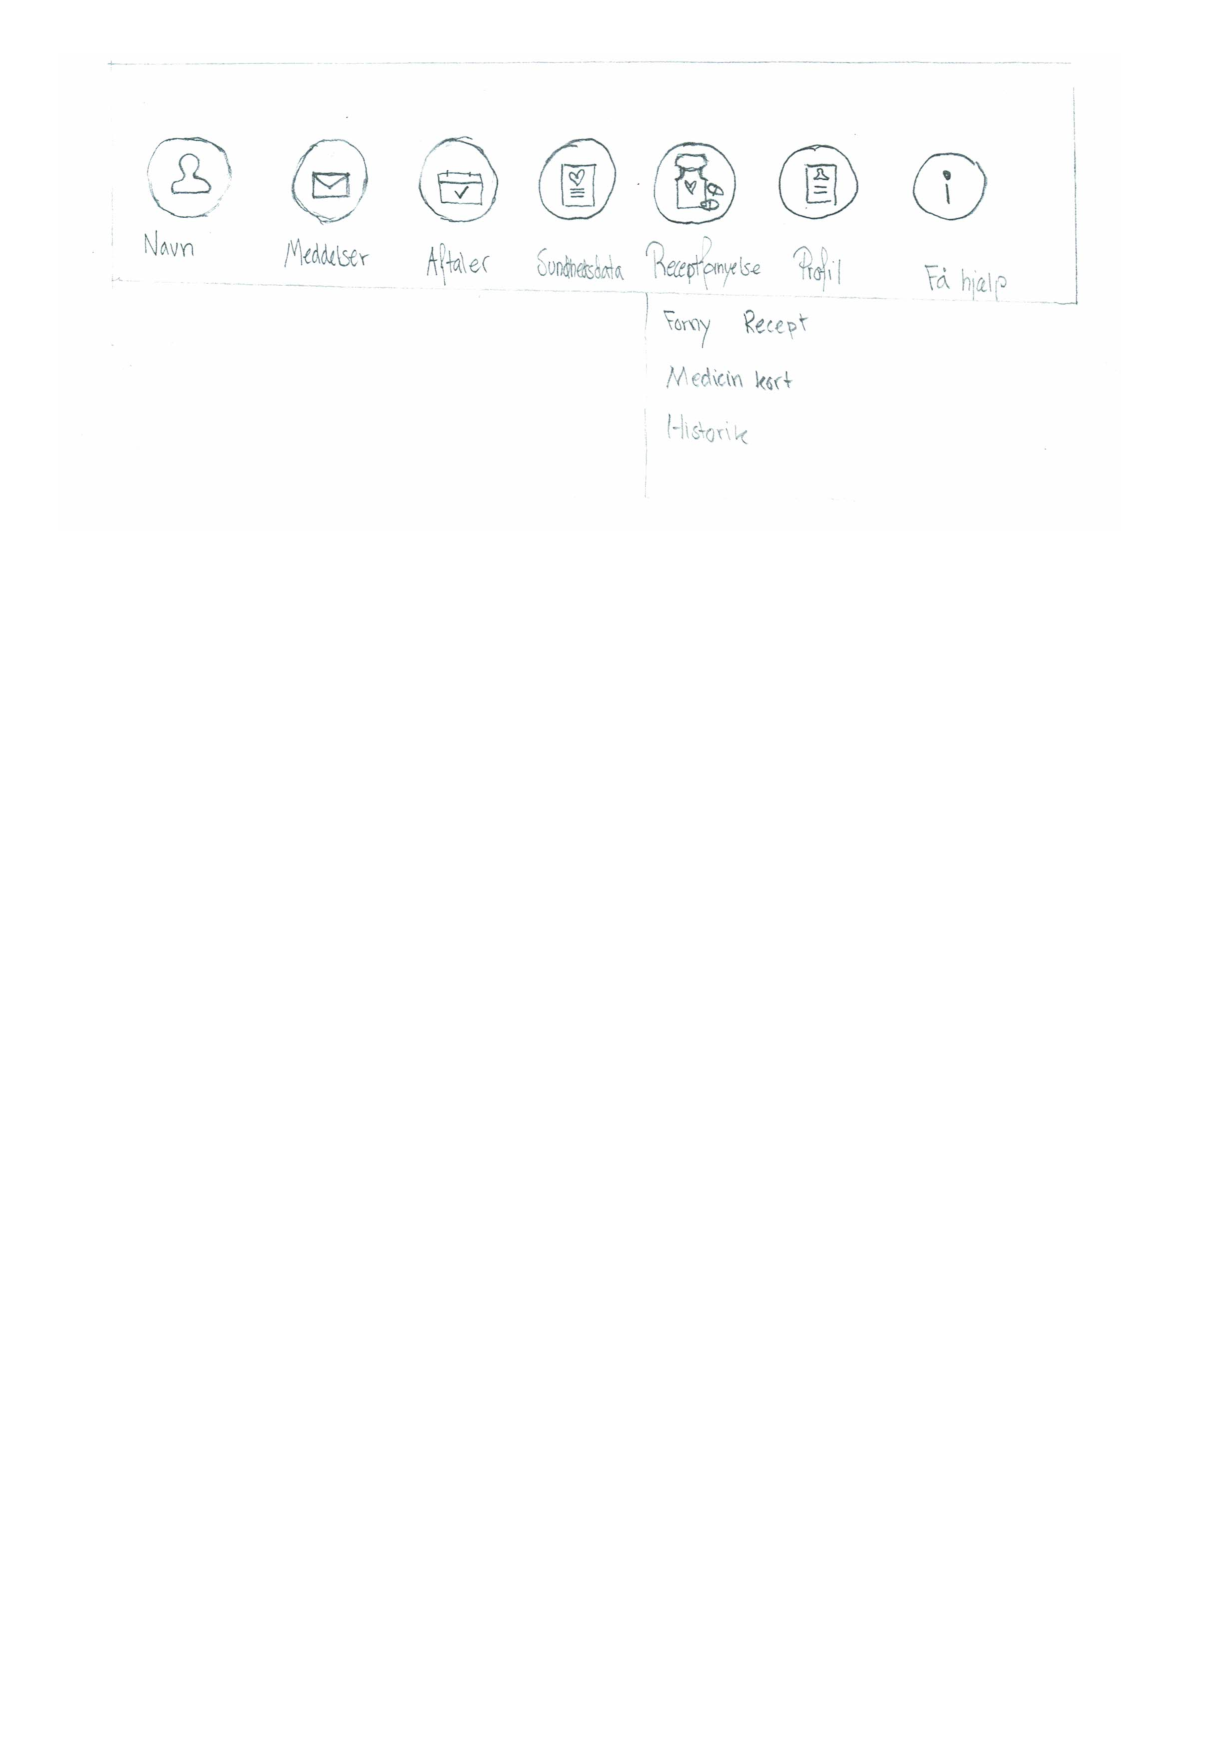
\includegraphics[angle=0, width=\linewidth]{Materials/FornyRecept_Hovedmenu.pdf}
	\caption{Mock-up for modulet 'Receptfornyelse': Hovedmenuen}
	\label{fig:Mock-Up1}
\end{figure}
Mock-up'en til Hovedmenuen med et 'Receptfornyelses-menu' er lavet med inspiration fra vores scenarier.\footnote{Bilag 5}
\begin{figure}[H]
	\centering
	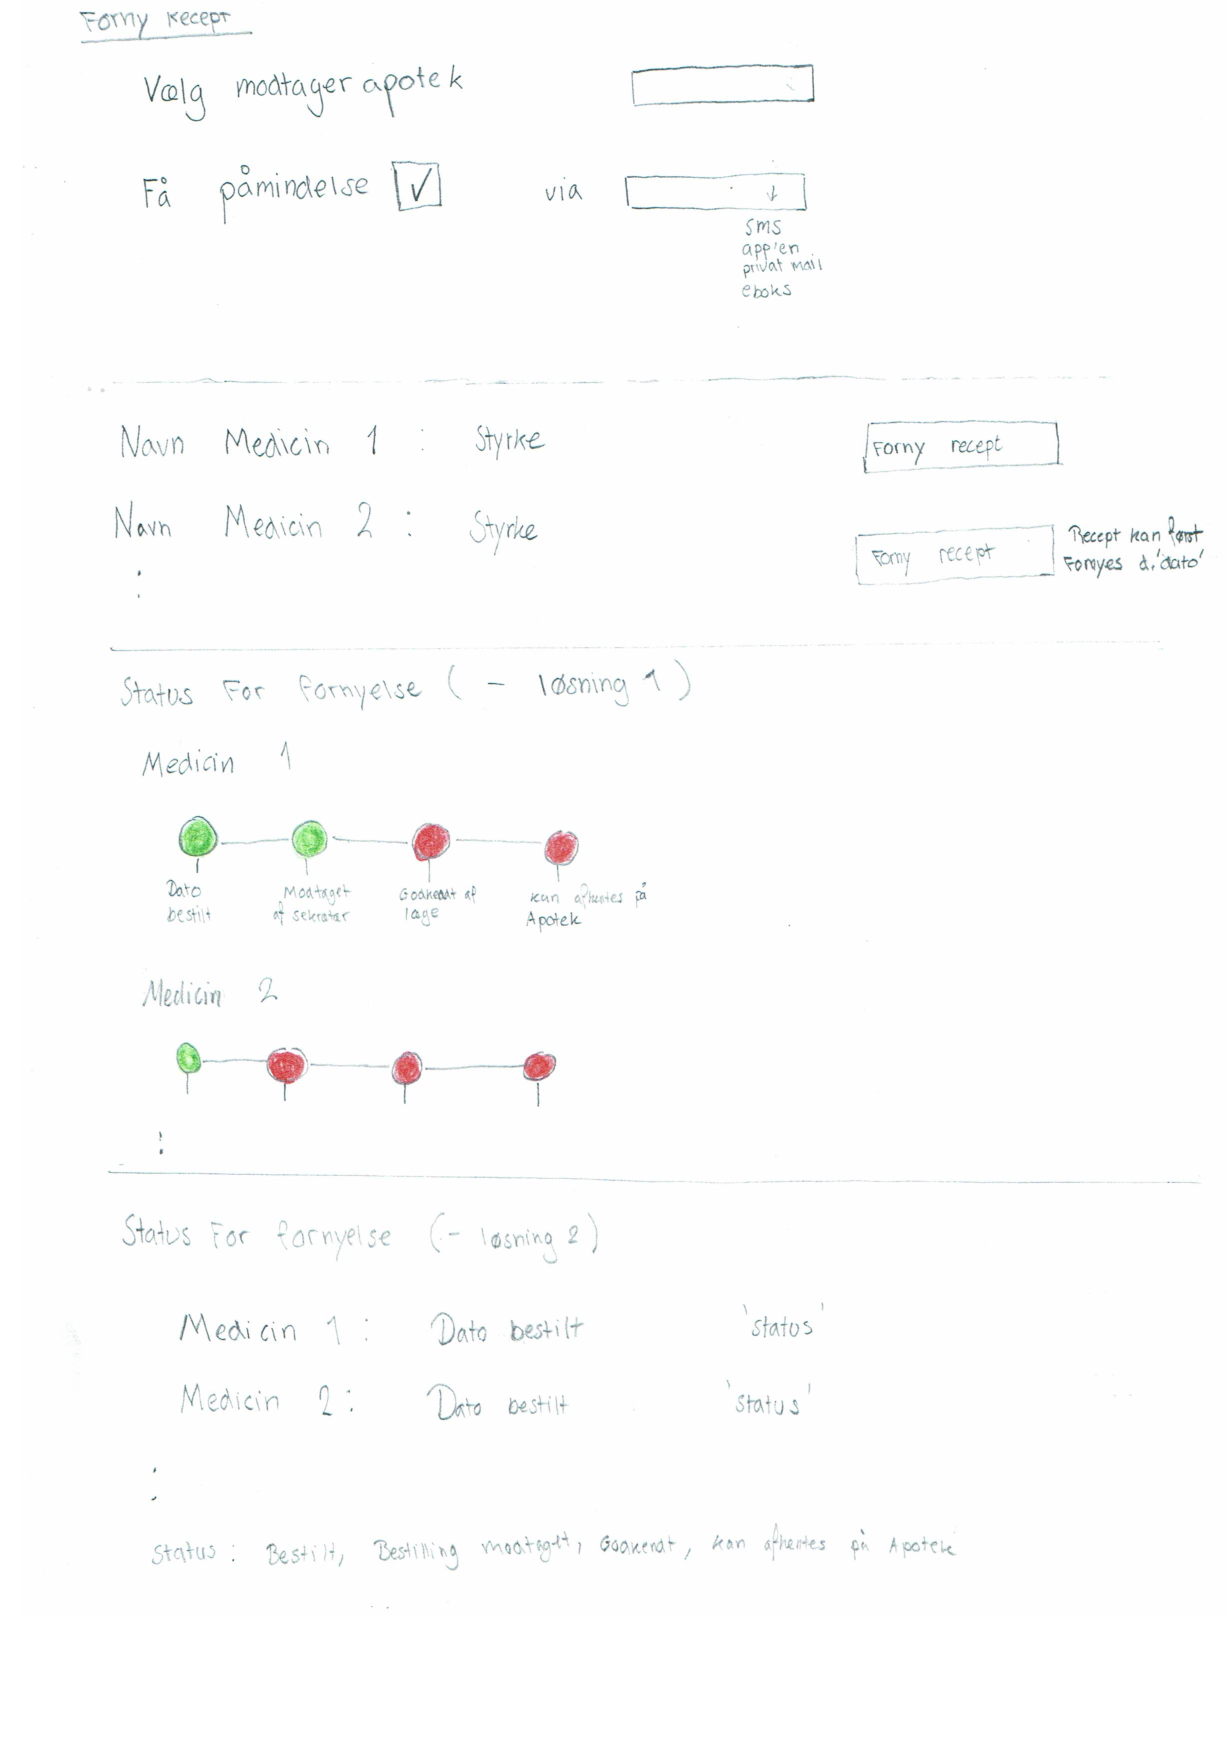
\includegraphics[angle=0, width=\linewidth]{Materials/FornyRecept.pdf}
	\caption{Mock-up for modulet 'Receptfornyelse': Undermenu, 'Forny recept'}
	\label{fig:Mock-Up2}
\end{figure}
I 'Vælg modtagerapotek' skal man i en drop-down menu kunne vælge mellem de to apoteker, som er tættest på en.\\
Hvis patienten ønsker påmindelse om receptfornyelse, skal patienten sætte hak ved 'Få påmindelse'.\\
Bemærk at knappen 'Forny recept' skal være blokeret i perioden, hvor recepten ikke må fornys. Der skal udover indformeres om, hvornår patienten igen kan forny sin recept, f.eks. med tekst ved siden af 'Forny recept'-knappen som vist i mock-upen.\\
Når patienten fornyer sin recept, skal der poppe en fortrydelsesbesked op, som siger: 'Er du sikker på du vil forny din recept?' hvor man skal kunne vælge 'Ja' eller 'Nej.\\
Der er to forslag til måden, hvorpå status for fornyelse kan vises. Statusmulighederne i løsning to er: Bestilt, bestilling modtaget, godkendt og kan afhentes på Apotek.\\
\begin{figure}[H]
	\centering
	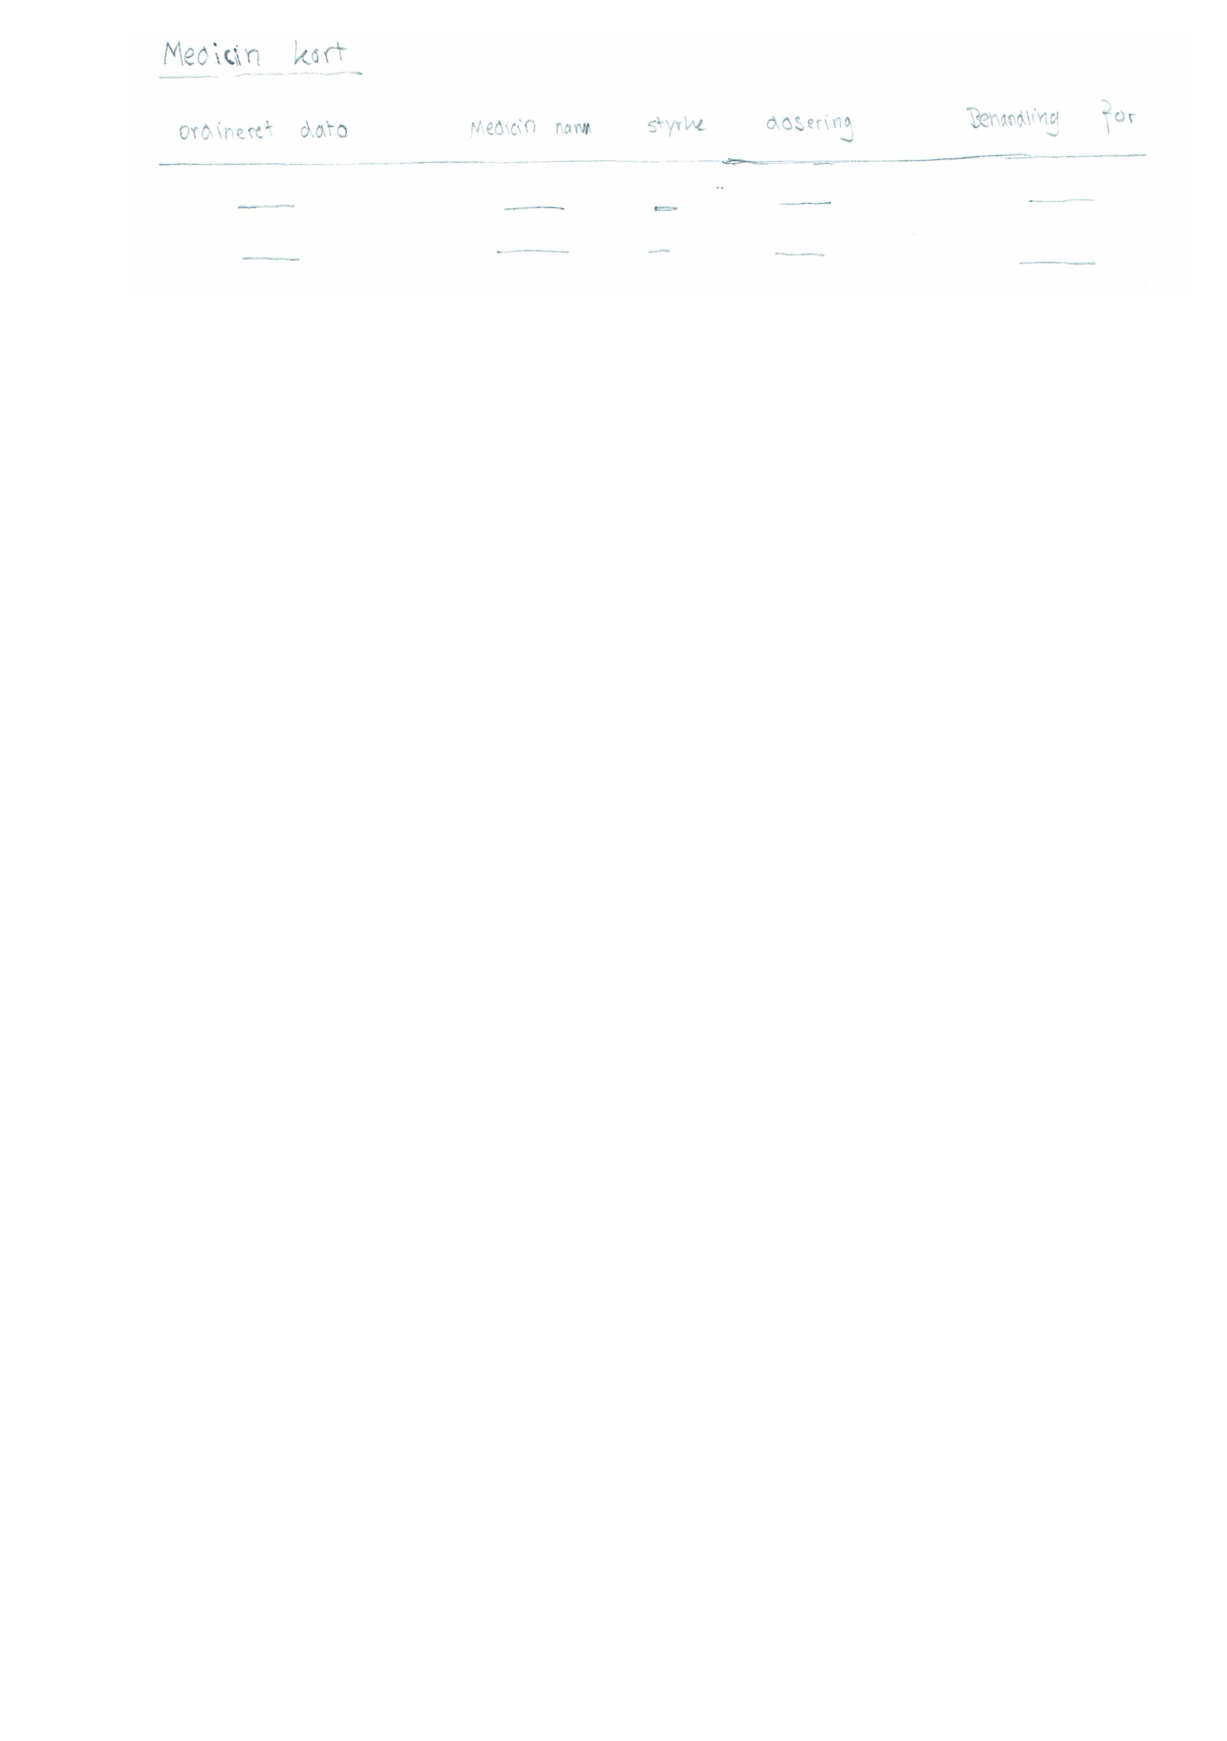
\includegraphics[angle=0, width=\linewidth]{Materials/FornyRecept_Medicinkort.pdf}
	\caption{Mock-up for modulet 'Receptfornyelse': Undermenu, 'Medicin kort'}
	\label{fig:Mock-Up3}
\end{figure}
\begin{figure}[H]
	\centering
	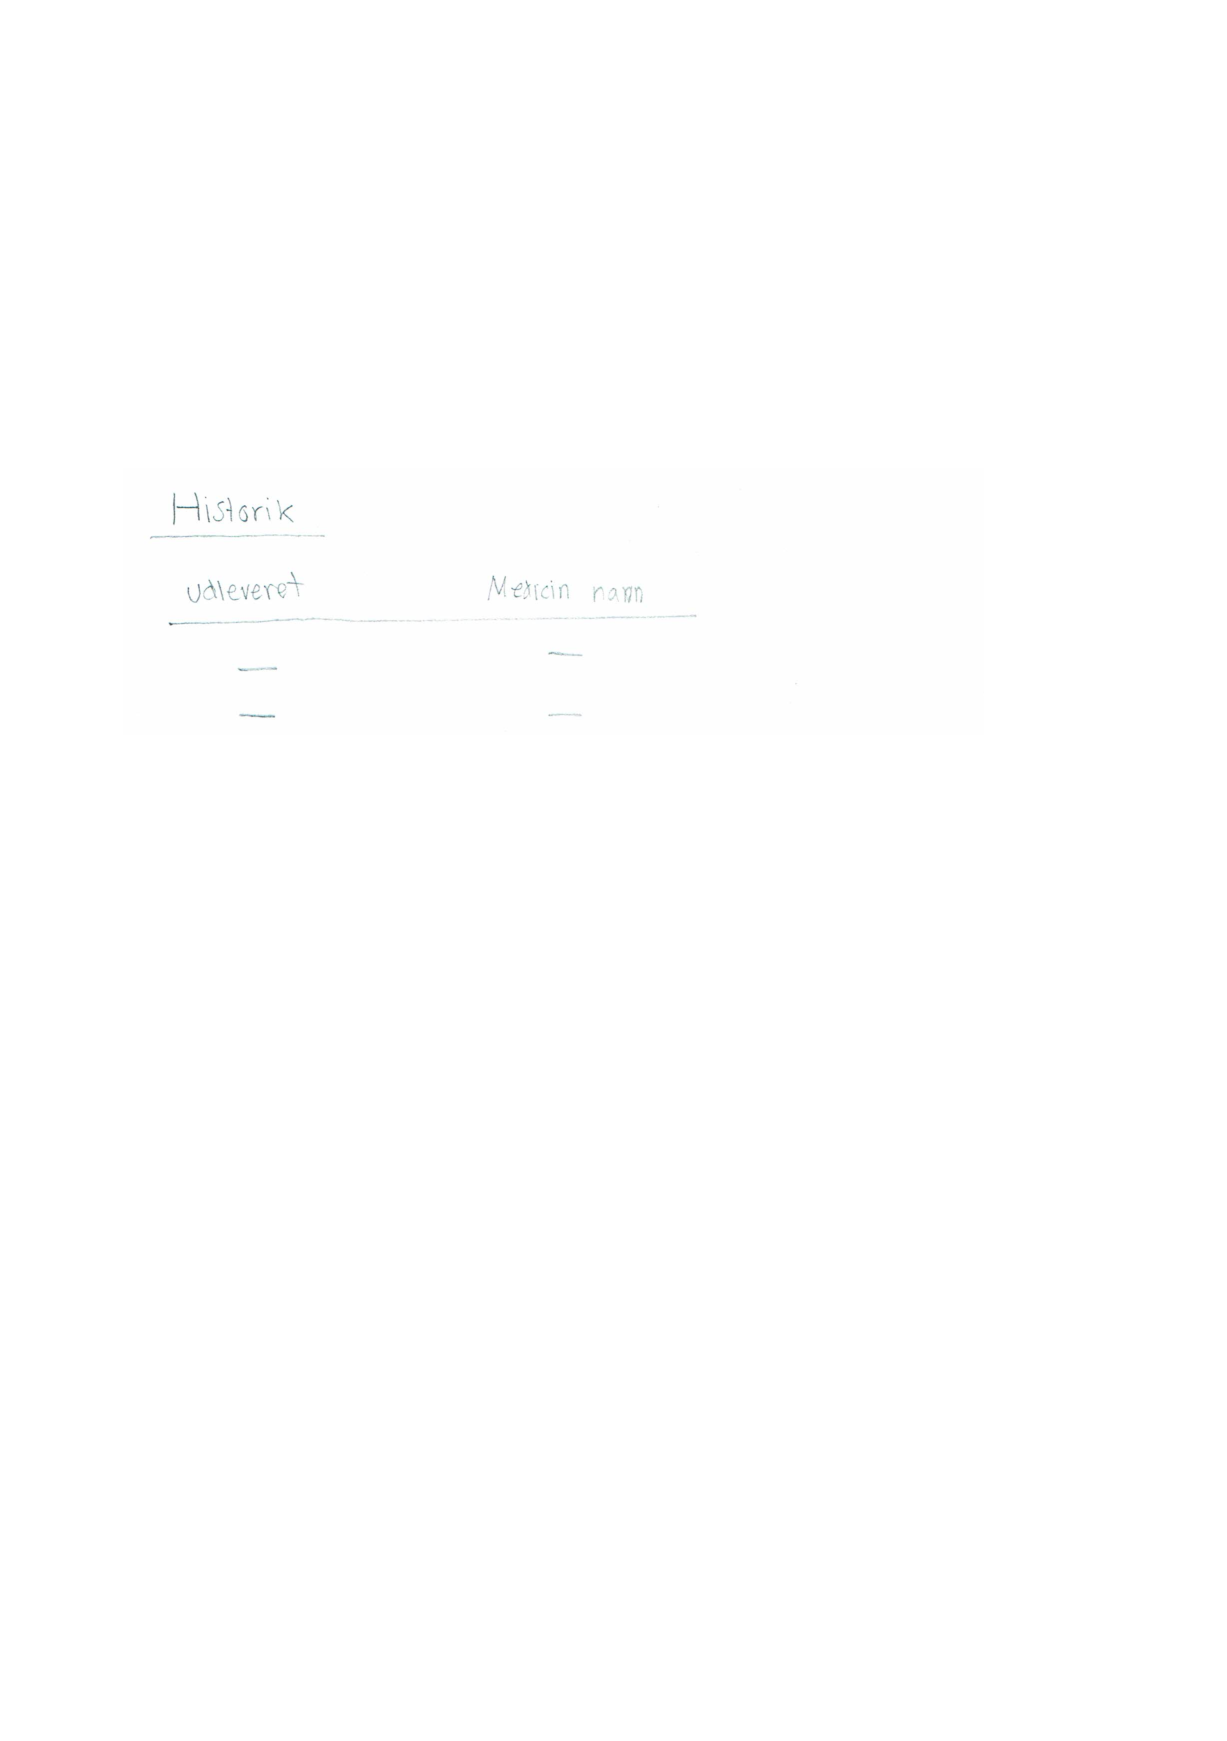
\includegraphics[angle=0, width=\linewidth]{Materials/FornyRecept_Historik.pdf}
	\caption{Mock-up for modulet 'Receptfornyelse': Undermenu, 'Historik'}
	\label{fig:Mock-Up4}
\end{figure}
% ? - Scenarios
\textbf{Samling af al information} \\
Forslag til brugergrænseflade for patienten fremgår af nedenstående Mock-up's:\\
\begin{figure}[H]
	\centering
	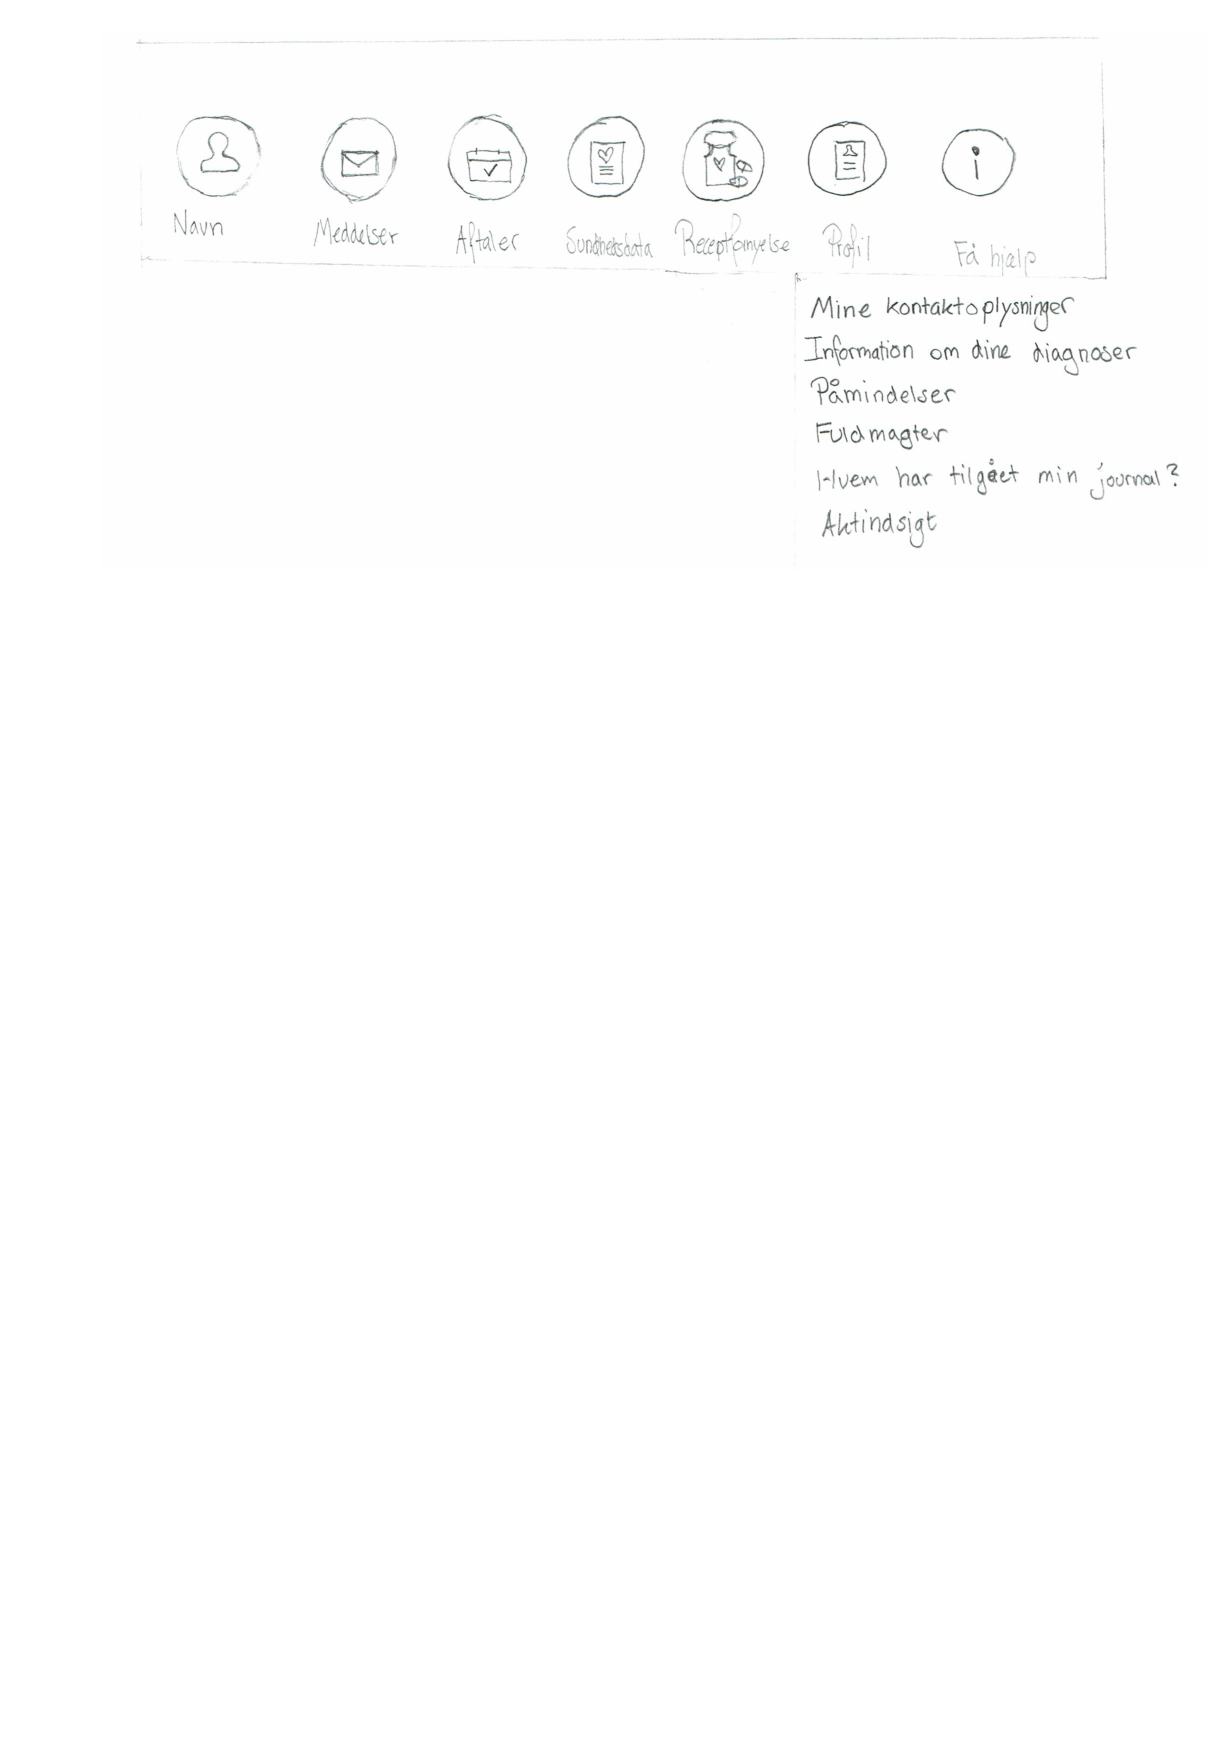
\includegraphics[angle=0, width=\linewidth]{Materials/Information_Hovedmenu.pdf}
	\caption{Mock-up for modulet 'Information om dine diagnoser': Hovedmenu, 'Profil'}
	\label{fig:Mock-Up5}
\end{figure}
Der er i hovedmenuen Profil tilføjet undermenuen 'Information om dine diagnoser'.
\begin{figure}[H]
	\centering
	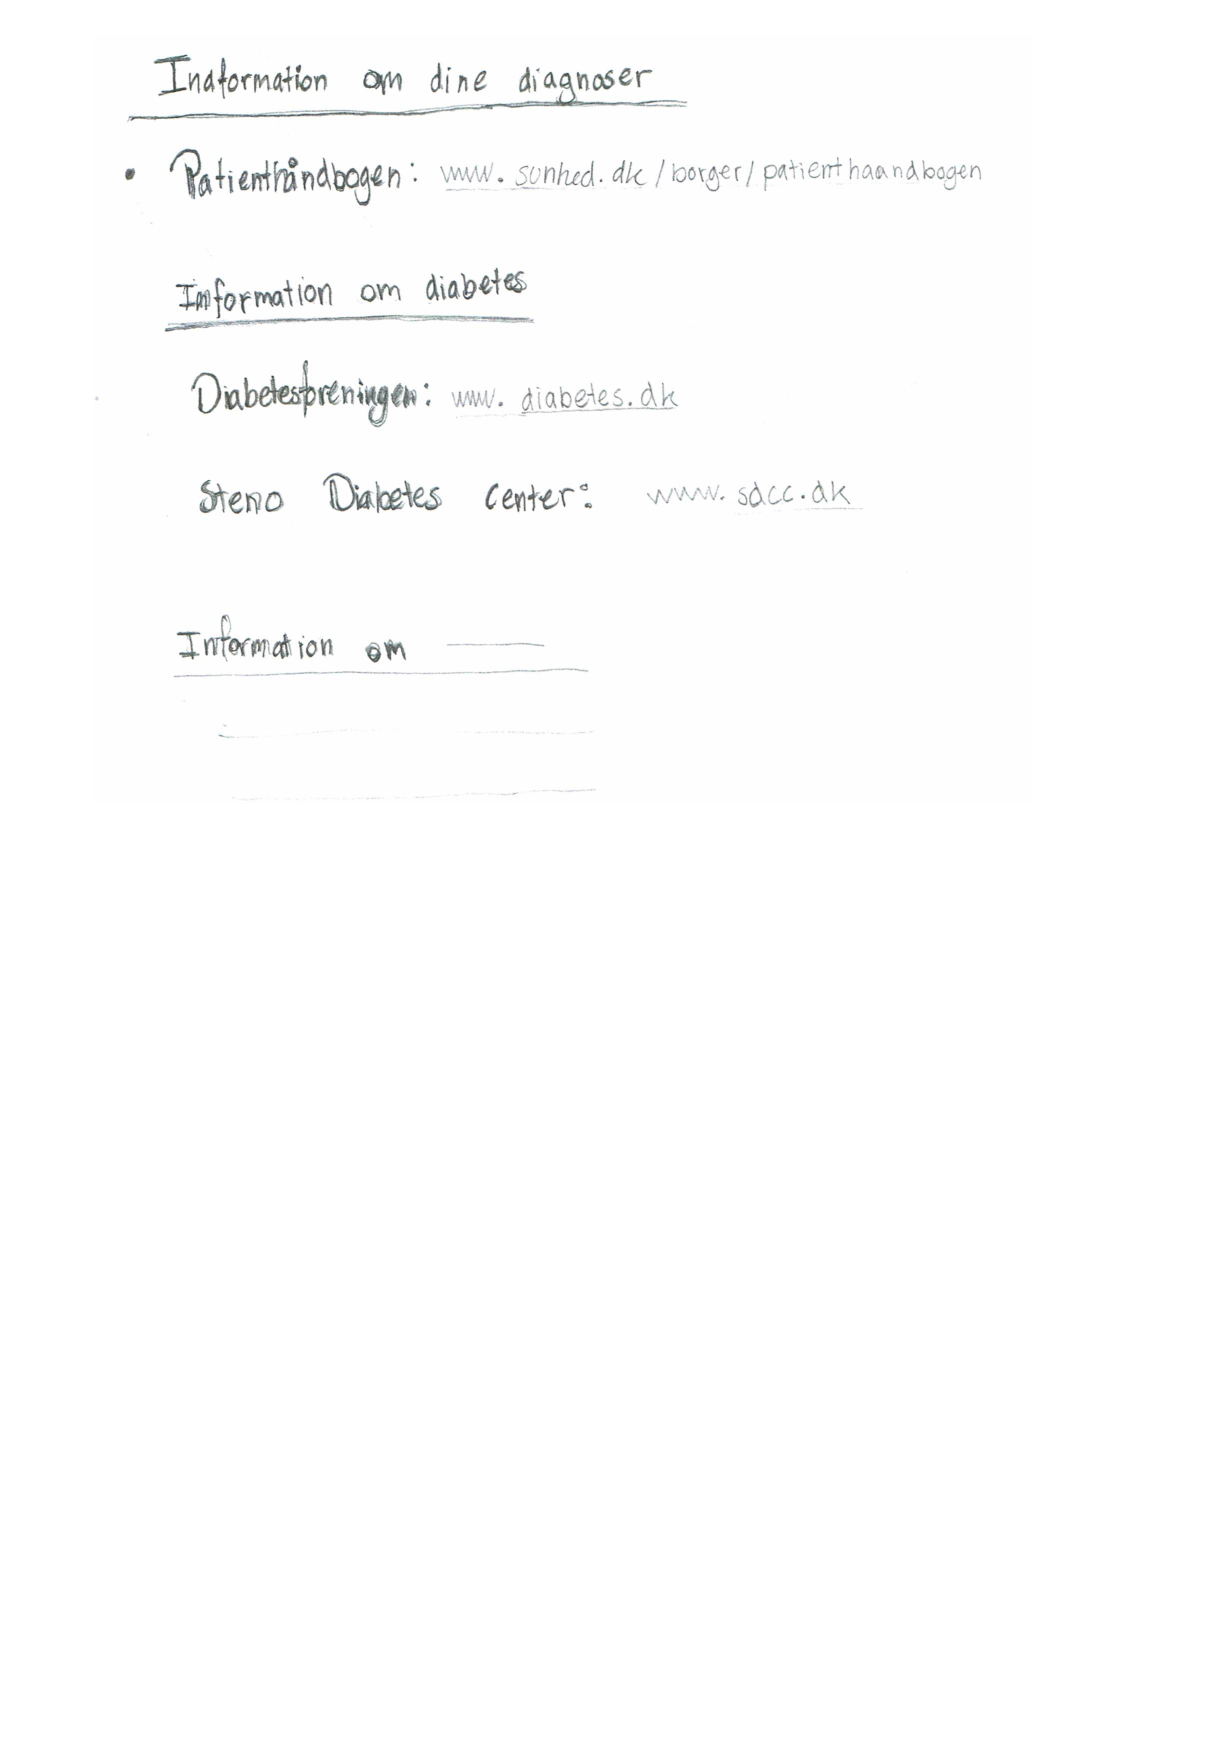
\includegraphics[angle=0, width=\linewidth]{Materials/Info2.pdf}
	\caption{Mock-up for modulet 'Information om dine diagnoser': Undermenu}
	\label{fig:Mock-Up6}
\end{figure}
Her kan patienten søge generel infomation om sin/sine diagnoser via links til relevante og anerkendte hjemmesider, der er udarbejdet af sundhedsfagligt personale.\\\\
\textbf{Uniforme Prøvesvar} \\
Forslag til brugergrænseflade for patienten fremgår af nedenstående Mock-up's:\\
\begin{figure}[H]
	\centering
	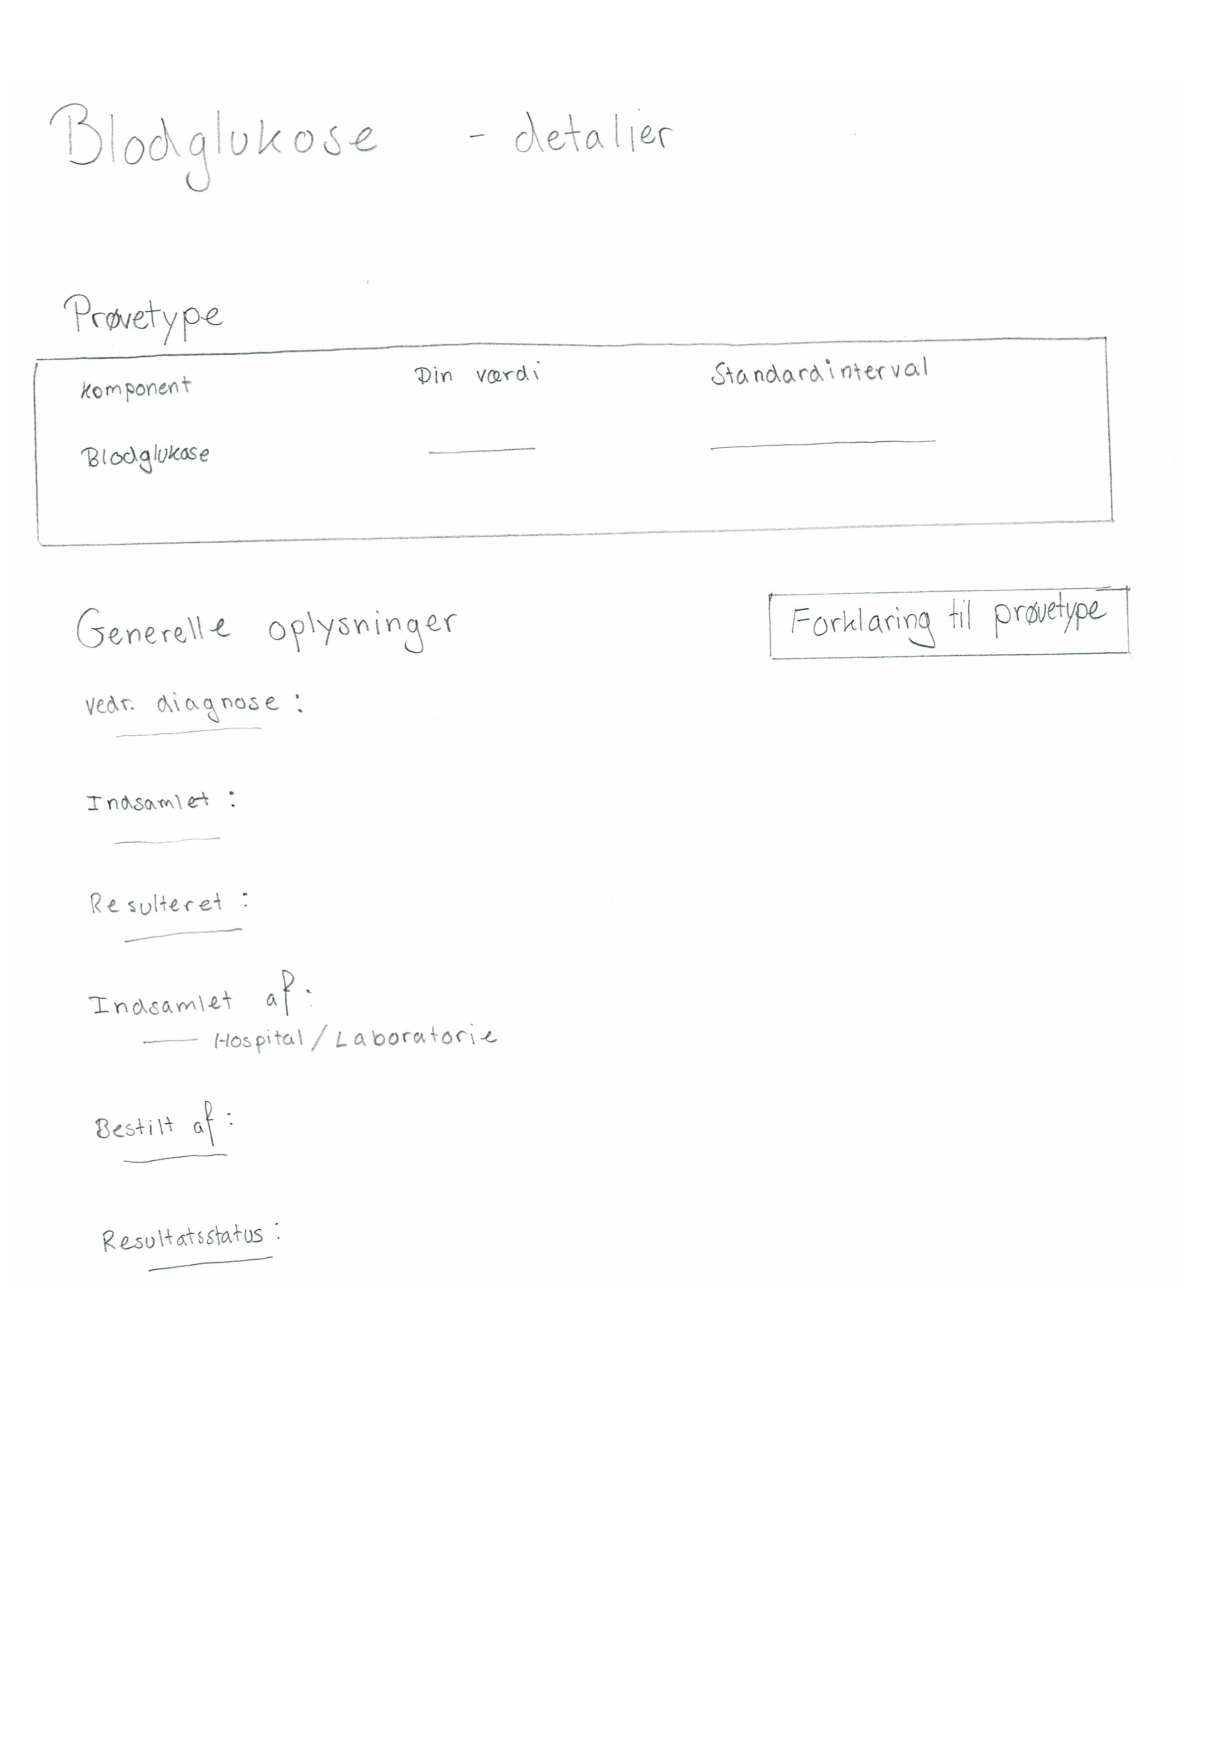
\includegraphics[angle=0, width=\linewidth]{Materials/provesvar.pdf}
	\caption{Mock-up for modulet 'Prøvesvar'}
	\label{fig:Mock-Up7}
\end{figure}
Når patienten klikker på knappen 'Forklaring til prøvetype' skal der vises en tekst på dansk med forklaringen til prøvetypen. Det kan laves som en pop-up eller ny side.\\

\subsection{Arbejdets organisering} 
Det lykkedes desværre ikke for os at få mulighed for at foretage virksomhedsbesøg. \footnote{Dybdeanalyse, afsnit 5 Konsekvensanalyse s. 18} Virksomhedsbesøg ville have givet os mulighed for at observere sundhedspersonalets nuværende arbejdspraksis, når patienterne fornyer deres recept via besked funktionen i MinSP og får taget prøver og givet prøvesvar.\\ 
Vi ville derfor bedre have kunnet vurdere hvilke ændringer, det giver i arbejdsorganisering for sundhedspersonalet og arbejdsfordelingen imellem læge, lægesekretærer, laboranter m.fl.\\
Vi havde også f.eks. haft mulighed for at observere forretningsgange, når patienterne bestilte receptfornyelse via sundhed.dk eller via en læges eget system, og fået inspiration til vores udvikling af receptfornyelse i MinSP.\\
Vi ville derfor have haft et bedre grundlag for at vurdere fordele og ulemper for sundhedspersonalet og relationerne imellem dem, deres arbejdsgange og evt. kvalifikationsbehov ved implementering af vores visioner.\\
Vi har derfor ikke haft den viden, som MUST-metodens princip om, at arbejdspraksis skal opleves ellers kunne have givet os. 
\\
\\
\textbf{Receptfornyelse} \\
En automatisk receptfornyelse vil muligvis ændre arbejdsgangen for sundhedspersonalet. \\ 
Lægen skal fortsat stadigvæk tjekke, at ordineringen er korrekt i forhold til journalen, men at læge-sekretæren slipper for at skrive besked tilbage til patienten, da patienten nu selv kan se forløbet i statuslinjen.
%
\\\\
\textbf{Samling af al information} \\
Hvis funktionaliteten implementeres via links som foreslået, vil der ikke være nogen ændringer til arbejdsgange og arbejdets organisering. \\
Hvis ikke funktionaliteten implementeres via links, men som en ny-udviklet informationside, er det sundhedspersonalet der skal skrive alt informationen/optage videoer mv., og siden vil skulle vedligeholdes af sundhedspersonalet, så det ville være en ekstra opgave, som sundhedspersonalet (læger, diætister og sygeplejeskær m.fl.) herved bliver pålagt.
\\\\
\textbf{Uniforme Prøvesvar} \\
Implementering af denne funktionalitet vil give ekstra arbejde for lægesekretæren eller laboratorie medarbejdere i forhold til indrapporteringen af prøvesvar, da der vil være flere informationer (navn på sted hvor prøven er taget og navn på diagnose), der skal indtastes, end med nuværende løsning. Der vil forinden være ekstra arbejde for lægen, da det er denne, der skal informere laboratorie-personale eller lægesekretær om, hvilken diagnose, de enkle prøvesvar vedrører.\\
Der skal tages stilling til hvor i organisationen indrapporteringen skal foretages. Desuden skal der nedsættes et udvalg enten på regionalt eller på landsplan som skal udarbejde standardsvarene til de uniforme prøvesvar.
\subsection{Kvalifikationsbehov}
\textbf{Receptfornyelse} \\
Receptfornyelses funktionaliteten vil ikke kræve nogen større oplæring af sundhedspersonalet, hvis de er rutinerede brugere af Sundhedsplatformen, men blot en introduktion til, hvordan den nye funktionalitet fungerer.
\\\\
\textbf{Samling af al information} \\
Hvis funktionaliteten implementeres via links, vil det ikke kræve nogen oplæring af sundhedspersonalet.
\\\\
\textbf{Uniforme Prøvesvar} \\
Vores vurdering er, at ændringerne ikke kræver ekstra kvalifikationer, da ændringen for sundhedspersonalet består i data-indtastning, som vi forudsætter at de allerede er bekendt med.
\\\\
Da vi ikke har haft mulighed for at foretage virksomhedsbesøg, har vi ikke haft kontakt med sundhedspersonalet i nogen af Region Sjællands hospitaler. Vi har derfor ikke haft mulighed for løbende at kunne informere personalet og ledelse om vores visioner til forbedring af MinSP som vi arbejdet med i dette forundersøgelses projekt. Vi har derfor ikke kunne opfylde MUST-metodens princip om forankring, hvor man fra forundersøgelsen første fase skal skabe forståelse og opbakning ved at informere alle interessenter der senere vil blive berørt af forandringerne. Det gælder både ledelse, sundhedspersonale og dem, der skal være ansvarlige for den tekniske og organisatoriske implementering.

% Konsekekvens-analyse resultatet giver Fordele og Ulemper
% ud fra Scenarios
%s. 207 Konsekvansanalyse: 'gennemgå systematisk de forslåene visioner'
%
%  Teknik: Virtuelle kort, evt. Brug SWOT s. 269-270, Design skitsere
%
% Pricippet Samlet Vision - s. 72 trekant:  IT-udvikling / kvalifikationsudvkling / Organisatoriske udvikling : 
%
%Diskution af
% hvad er ændringen
% hvordan pårvirker det mennesker der skal bruge det
% Arbejds Organiserings ændringer / skaber det ændringer i arbejdsgange
% Forankring ('knytter sig til' personalet og organiserings)
% krav til uddanelse /kvalifikations krav
% Økonomi
% /Matcher det med Region H. forretnings og IT stategi
\section{Konsekvensanalyse: Fordele og Ulemper}
I dette afsnit ser vi på hvorfor visionerne er relevante for Region Sjællands forretnings- og it-strategi, for sundhedspersonalet og for patienter og lervandører. \\
Til hjælp i vores vurdering af fordele og ulemper af visionerne om 'Receptfornyelse' og 'Samling af al information' på MinSP, har vi udarbejdet to scenarier, hvor visionerne ses ud fra henholdsvis en bruger og en sundhedsfagligs synspunkt. Scenarierne ses nedenfor under \textcolor{red}{punkt 6}.
\todo{Virtuelle kort / SWOT analyse}
\subsection{Region Sjællands forretnings- og it-strategi}
\textbf{Prioritet 1, Receptfornyelse}\\
Fordelen ved at implementere en automatisk receptfornyelses funktionalitet er, at brugerne kan betjene sig selv og vil opleve en bedre service. Det vil muligvis også reducere sundhedspersonalets ressourceforbrug. Dette opfylder målsætninger i Region Sjællands it-strategi \footnote{Projektgrundlag, s. 6, Afsnit 3.1 IT strategien, punkt 7 }.\\
Det vil også opfylde Region Sjællands it-strategi om infrastruktur, at MinSP bliver en samlet side for alle funktioner og har integrerede selvbetjenings løsninger. \footnote{Projektgrundlag, s. 7, Afsnit 3.4 It-infrastruktur punkt 3 og 4}\\
Ulempen er, hvis funktionaliteten 'Receptfornyelse' ikke bliver brugt af patienterne, men at patienterne i stedet stadigvæk bruger sundhed.dk, fordi vi vuderer, at funktionaliteten vil være rimelig dyr at implementere, og det vil være i modstrid med Region Sjællands it-strategi om at "Regionen vil have fuldt udbytte af sine investeringer, og de nye løsninger skal bruges i deres fulde omfang" \footnote{Projektgrundlag, s. 5, Afsnit 3.1 IT strategien, punkt 2}. Det vil sige, at det så vil være en dårlig cost/benefit for regionen.\\ 
En bedre løsning ville så være kun at oprette den nye hovedmenu 'Receptfornyelse' og herunder linket til sundhed.dk. Det vil dog være i modstrid med Region Sjællands it-infrastruktur, om at "Brugeren skal kunne finde løsninger i samme brugervendte arbejdsgange, uden at brugerne skal opleve behov for at navigere mellem forskellige løsninger" \footnote{Projektgrundlag, s. 7, Afsnit 3.4, It-infrastruktur, punkt 3}. 
\\\\
\textbf{Prioritet 2, Samling af al information}\\
En 'standardløsning' med link til sider med information om diabetes stemmer overens med Region Sjællands forretnings- og it-strategi om, at patienter i så høj grad som muligt skal kunne betjene sig selv samtidig med, at de får en bedre servicegrad og regionen reducerer sit ressourceforbrug. \footnote{Projektgrundlag, s. 6, Afsnit 3.1 IT strategien, punkt 7} \\
Det er også en prioritet i it-strategien, at systemer skal kunne hente information fra andre systemer, så dette understøttes også af vores løsning. \footnote{Projektgrundlag, s. 6, Afsnit 3.1 IT strategien, punkt 8} \\
Løsningen opfylder også en målsætning i regionens it-infrastruktur om at: "Regionen ønsker systemer, som kan hente information fra andre systemer, således at brugeren kun skal henvende sig et enkelt sted".\footnote{Projektgrundlag, s. 7, Afsnit 3.4 It-infrastruktur, punkt 3}
\\\\
\textbf{Prioritet 3, Uniforme Prøvesvar}\\ % ? - Er løsningen dyr at kode
En forbedret løsning til visning af prøvesvar vil give patienterne bedre service som er i overensstemmelse med regions it-strategi. \footnote{Projektgrundlag, s. 6, Afsnit 3.1 IT strategien, punkt 7}\\
Det er det sundhedsfaglige personale, der skal lave de danske beskrivelser for de forskellige typer af prøvesvar. Dette matcher ikke med Region Sjællands ønske om at reducere sit ressourceforbrug \footnote{Projektgrundlag, s. 6, Afsnit 3.1 IT strategien, punkt 7}, så cost/benefit skal vurderes i forhold til det forbedret service niveau for patienterne. 
\subsection{Relationer mellem sundhedspersonalet og mellem afdelinger}
\textbf{Prioritet 1, Receptfornyelse}\\
Det er en fordel for læge-sekretærerne, at de ikke længere skal huske at svare tilbage til patienter omkring receptfornyelse og skal bruge tid på det.
% Ulemper -?
\\\\
\textbf{Prioritet 2, Samling af al information}\\
Det er en fordel for sundhedspersonalet, at patienterne i højere grad selv kan søge information, da det vil betyder mindre arbejde for sundhedspersonalet.\\
Det vil give en bedre kommunikation mellem sundhedspersonalet og patienterne, når patienter, via informationslinksene, er bedre informeret om deres sygdom, behandlingsforløb, kost og motion m.v.
% Ulemper -?
\\\\
\textbf{Prioritet 3, Uniforme Prøvesvar}\\
Prøvesvarene bliver mere forståelige for patienterne, og det vil lette arbejdet for sundhedspersonalet med at besvare spørgsmål og forklare prøvesvar for patienterne.\\
Det er en ulempe, at sundhedspersonalet får mere arbejde med at indrapportere ekstra data. \\ Det er også sundhedspersonalet, der skal lave de danske tekster.
\subsection{Patienter og lervandørere}
\textbf{Prioritet 1, Receptfornyelse}\\
Patienter kan bestille receptfornyelse det samme sted, som hvor de kan se prøvesvar og kommunikere med hospitalet, og de kan følge med i, hvor langt deres bestilling er nået.\\
Det kommer muligvis til at gå hurtigere for patienten at få fornyet sin recept, fordi der ikke skal skrives beskeder til hospitalet. Patienten undgår arbejdet med at skrive beskeder og at skulle huske, hvad medicinen hedder.\\
Patienten får også et medicin kort, der er nemt at finde og adgang til en historik over, hvad de har fået af medicin gennem tiden i deres sygdoms forløb.\\
Der tages hensyn til brugervenligheden ved at gøre receptfornyelses modulet synligt.\\ 
Der er ingen ulemper for patienten, for de vil stadigvæk kunne bruge sundhed.dk eller kunne kontakte egen læge, hvis de hellere vil det.\\
Apoteket vil muligvis komme til at skulle tjekke to steder for medicin bestilling: sunhed.dk og MinSP.
\\\\
\textbf{Prioritet 2, Samling af al information}\\
Ifølge vores interview-undersøgelse har det at kunne søge information og vejledning om sin sygdom været meget efterspurgt. Så løsningen vil opfylde et stort behov hos brugerne. \\
Linket til patienthåndbogen er gjort mere synlig ved at være flyttet fra "Historik" under "Sundhedsdata" til "Information om dine diagnoser" under "Profil". Det har gjort informationssøgning på MinSP mere brugervenlig for patienterne.\\
Vi har udvidet med to ekstra informationslink, hvor patienterne kan finde information om nogen af de forhold de har efterspurgt, f.eks. video om hvordan man måler blodglukose, kost-vejledning mm.\\
Det er nemt at udvide modulet med flere informationssider, hvis dette ønskes af patienterne.\\
Der skal muligvis skaffes tilladelse fra leverandørerne af linksene til at bruge linksene.
% Patienter og levandørere: de skal sige god for til links i 'Samling af al information'
\\\\
\textbf{Prioritet 3, Uniforme Prøvesvar}\\
Patienterne vil bedre kunne forstå, hvad et prøvesvar omhandler, når der er tilknyttet en standard beskrivelse på dansk. Patienten vil også kunne se, hvor deres prøver er taget.\\ Begge tilføjelser er, jf. vores interviews, et ønske fra patienterne.\\
Ved at samle prøvesvarene pr. diagnose giver det patienterne et bedre overblik over deres prøvesvar.
\subsection{Finanser}
At implementere vores visioner til en fyldestgørende grad ville være en dyr affære med behov for programmører og andre designere, som regionen og/eller staten skal finansiere. Evt. ville jobbet skulle outsources til et firma som det amerikanske Epic, der oprindeligt implementerede Min Sundhedsplatform. Dette ville skulle gøres uden udsigt til indtægt, da Min Sundhedsplatform er udelukkende gratis og der derfor ikke er mulighed for at tjene penge ind igen på investeringen og den yderligere service såsom receptfornyelse, passer ikke naturligt med at kræve betaling fra brugeren. Dette er essentielt at medbringe i overvejelserne, når man skal beslutte at lave disse tilføjelser eller ej. 

\section{Strategi og plan for implementering}
I dette afsnit ønskes at bygge et grundlag for, hvorledes vores visioner kan realiseres.
Dette indebærer forskellige faktorer, som i følgende vil undersøges:
\begin{itemize}
  \item En forståelse for projektets omfang. Her vil eksempelvis receptfornyelse igennem Min Sundhedsplatform involvere læger og deres interne systemer i hele region Sjælland og Hovedstaden, hvilket bidrager til projektets store omfang. Under samme ovevejlser tilhører projektets finanser. Det store omfang medfører naturligvis en stor omkostning, som skal finansieres af regionen og det skal evalueres, hvorvidt vores visioner er den økonomiske investering værd. 
  \item En forståelse for diverse risici og eventuelle konflikter, som kunne hindre projektet. Dette inkluderer f.eks. besværlige, interne systemer hos lægerne, der kræver ekstra arbejde at koble på Min Sundhedsplatform, og hvis dette ikke virker, vil det i værste tilfælde efterlade nogen ude af stand til at benytte den nye funktionalitet til at fornye deres måske vigtige medicin, hvorfor risiko-faktoren er høj for dette projekt. 
  En måde vores plan ville kunne håndtere tilstedeværelsen af diverse fejl og konflikter, er ved efter endt pilot-projekt at lave evaluering af denne, således at kritiske fejl opdages tidligt i processen, hvor de er relativt billige at løse kontra senere i processen.  
  %\item En overordnet fremgangsmåde til projektets realisering. Denne bestemmes ud fra en analyse af både projektets risici, omfang og tidsbegrænsninger. Hvis tid tillader det, da vil en inkremental fremgangsmåde muligvis vise sig optimal, da en gradvis implementation af alle dele af projektet er med til at sikre en høj kvalitet af og sammenhæng mellem disse.
  \item En dybdegående analyse af diverse involverede parter og deres interesse i projektet, hvilket kan tage udgangspunkt i afsnittet om scenarier, der giver indblik i netop dette. 
\end{itemize}

For vores tre prioriteringer (uniforme prøvesvar, receptfornyelse og samling af information på Min Sundhedsplatform), ønsker vi konkret følgende:
\begin{itemize}
	\item Til uniforme prøvesvar vil det primære problem ligge i den administrative process, som det ville kræve at komme til enighed omkring de uniforme prøvesvars form. Mere konkret ville samrådet blandt diverse hospitaler i regionen/landet skulle komme til enighed om dette for at opnå det ønskede resultat. Omend billigt på implementations-fronten, ville dette især være en tidskrævende, administrativ og bureakratisk proces. 
	\item Til receptfornyelse over Min Sundhedsplatform, ville der skulle laves et system, som kan interagere med diverse lægers allerede eksisterende, interne systemer. Da lægernes interne systemer ikke er garanteret at følge nogen standard, kan disse variere meget, hvorfor en implementation for at interagere med disse over Min Sundhedsplatform ville være en dyr affære at implementere. En plan til denne implementation ville være at skabe et pilot-projekt for at sikre, at de mest kritiske fejl og mangler opdages tidligst muligt i processen og derefter påbegynde en inkrementel strategi, som kan forløbe henover et års tid for at indfase regionens patienter.   
\textcolor{red}{\\
	S: Til det overstående:\\	
	Lægerne på hospitalet har ikke et intern system de bruger den del af SP som de har en adgangs rettighed til. \\
	Der er allerede integration mellem MinSP og SP.\\
	Recepten laves i SP. (Jf. Kaalund).	\\
	\\
	Der skal dog laves en forbindelse til FMK - da MinSP ikke har integration med FMK.\\
	- Se: Interview med Mette Christensen \\
	\\
	I kan også diskuteres en plan for at recept-systemet skal "vide" hvilken afdelingen på hospitalet recepten skal sendes til.\\
	\\
	- Se igen: Interview med Mette Christensen\\
	\\
	Hvis det er privat læger I snakker om har hverken Region Sjælland eller vi en målsætning om at få SP og MinSP ud til privatlæger p.t.\\
}
	\item Til samling af 
	\textcolor{blue}{al} information på Min Sundhedsplatform, \textcolor{red}{S: Her fra og til '..gennemgå det for faktuel korrekthed' bør slettes da det både er en gentagelse fra Konsekvensanalysen' og ikke er den løsning vi går med.} skal der sikres en høj kvalitet og korrekthed af denne information, da processen ellers havde været spild og endda være en dårlig tilføjelse, hvis Min Sundhedsplatform misinformerede patienter. Derfor skal en læge eller anden relevant sundhedsfaglig person ente selv skrive informationen eller gennemgå det for faktuel korrekthed. Alternativt \textcolor{red}{S: I skal ikke skrive 'Alternativt' - I skal kun skrive om løsningen med link - ellers matcher vores rapport ikke sammen.}  kan Min Sundhedsplatform linke til eksterne sider såsom steno.dk, hvilket dog ikke løser problemet med at garantere korrektheden af informationen
	\textcolor{red}{S: Hvorfor garanterer det ikke korrekthed - Steno er førende indenfor diabetes. De er absolut meget troværdige.}. Den dyre del af at implementere dette, ville derfor være den tidskrævende process at fakta-checke information.
	\textcolor{red}{S: Jeg mener ikke det skal faktatjekkes. Hvad lægerne derfra har skrevet, behøver ikke at blive fakta tjekket af andre læger.
	}
\textcolor{red}{\\\\S: Husk vi har skrevet at vi kun lægger sider op til diabetikere der har en lægefaglig baggrund - det gælder de tre sider der bliver nævnt: diabetesforeningen, patienthåndbogen og steno.}
\end{itemize}
Under udvikling af receptfornyelsesmodulet, vil hospitalerne ikke have nogen arbejdsbyrde, da implementationen af dette ligger eksternt fra hospitalerne selv.
\textcolor{red}{S: Hvordan skal det udbyde eksternt - kan I skrive noget mere omkring det - skal det i udbud mv. (Hvordan er forløbet?) - Kan dette muligvis uddybes mere?} Ligeså vil arbejdet på uniforme prøvevar ikke belaste hospitalerne, da et samråd mellem hospitalerne i denne periode skal bestemme naturen af de uniforme prøvesvar, hvilket er udelukkende administrativt arbejde. I denne periode ville det derfor være oplagt at påbegynde arbejde med samling af information
\textcolor{blue}{S: erstat 'samling af information' med: 'vurder og beslutte hvilken links der skal indgå i forhold til forbedringsforslaget 'Samling af al information'}
\textcolor{red}{S: Det andet kan misforstås - og vores rapport skal matche.}
 på Min Sundhedsplatform, da de andre processer i denne periode ikke belaster hospitalerne. Det er forventeligt, at udvikling af receptfornyelse ikke nås færdiggjort forinden, at 
 \textcolor{blue}{forbedringsforslaget} samlingen af 
 \textcolor{blue}{al} information på Min Sundhedsplatform realiseres. Når udvikling af receptfornyelsesmodulet så er færdiggjort, ville næste led i planen være at påbegynde pilot-projektet og derefter inkrementel-strategien for at realisere visionen om det ønskede receptfornyelsesmodul.
Når den beaukratiske proces i samrådet mellem hospitaler er færdiggjort, skal den implementeres, hvilket sker ved at lægerne og andet sundhedsfagligt personale informeres i den besluttede standard, så den fremover benyttes. Dette forventer vi sker midtvejs i processen om realisering af vores receptfornyelsesmodul.

\section{Prototype}
I de følgende afsnit vil vores prototype blive gennemgået. Først gennemgås vores ER-diagram og hvordan vi er kommet frem til vores endelige tabeller i databasen. Deri er en overordnet gennemgang af hvordan entiteterne i ER-diagrammet hænger sammen med vores forbedringsforslag om receptfornyelse, og hvilke features vores prototype understøtter. Dernæst gennemgås hvordan vores flask applikation er sat op, hvordan den køres og hvordan man kører vores tests. Efterfølgende er en showcasing af prototypen og de understøttede features, og afslutningsvis har vi en liste af known shortcommings.

\subsection{Model}
Ud fra vores vision om et receptfornyelsesmodul, vores udarbejdede user stories og vores MoSCoW prioriteringer har vi udviklet nedenstående ER-diagram over vores domæne.\\
\missingfigure{ER diagram}\\
Vores recept entitet kan unikt identificeres ud fra vores andre entiteters nøgler, og er derfor lavet en weak entity. Blandt vores ønskede funktioner er historik og medicinkort. Da der i en log over historik godt kan fremstå den samme medicin til den samme patient flere gange, har det været nødvendigt at tilføje en 'Historik' entitet som udover ovennævnte kan holde tidspunktet for fornyelsen af recepten.\\
Medicinkortet kan 'laves' ud fra recept entiteten givet hvilken patient der ønsker at se sit medicinkort. Det har derfor ikke været nødvendigt at lave en entitet til denne feature.\\

Vi har herefter omsat vores entiteter til tabeller på samme hvis som beskrevet i \textit{'Database Systems. The Complete Book'}\footnote{Prentice Hall, Database Systems. The Complete Book, s. 157-163}. Mange af vores entiteter kan laves direkte til en tabeller som ses nedenfor:
\begin{align*}
	&\textrm{Patient}(\textrm{\underline{CPR}, Password})\\
	&\textrm{Apotek}(\textrm{\underline{Navn}, Addresse})\\
	&\textrm{Medicin}(\textrm{\underline{Navn}, \underline{Styrke}})\\
\end{align*}
Ligeledes kan 'Diagnose' laves direkte. Denne tabel vil komme til at indeholde alle de diagnoser som kan gives, og er nødvendig da en patient kan have mere end en diagnose.\todo{High potential for change}
\begin{equation*}
\textrm{Diagnose}(\textrm{\underline{Sygdom}})
\end{equation*}
Vi har herefter vores 'Recept' entitet. Denne er weak, og henter nøgler fra de fleste andre entiteter. 'Status' attributten vil blive benyttet i overensstemmelse med vores vision om at patienten selv skal kunne følge med i receptfornyelsesprocessen. 'Udstedt' attributten vil blive benyttet af medicinkortet, og vil aldrig ændre sig da den repræsenterer hvornår patienter første gang blev ordineret med medicinen. 'Udløber' attributten vil blive benyttet til at sende reminders til patienterne.\todo{For detaljeret? Nogen grund til at forklare disse attributter?} 
\begin{equation*}
	\textrm{Recept}(\textrm{\underline{ApoNavn}, \underline{MedNavn}, \underline{MedStyrke}, \underline{PatCPR}, \underline{fornyet}, status, udstedt, udløber})
\end{equation*}
Hvis vi skulle lave vores relationer til om til tabeller ville der blive en en masse redundancy da alle på nær en enkelt relation vil allerede være subsets af andre tabeller. Derfor er den eneste relation som bliver lavet om til en tabel 'Behandles for'. Her vil begge nøgler være foreign keys til henholdsvis 'Patient' og 'Dignose'.
\begin{equation*}
\textrm{BehandlesFor}(\textrm{\underline{PatCPR}, \underline{Sygdom}})
\end{equation*}
\subsection{Prototype Flask}
Vores Flask applikation tager udgangspunkt i \textit{'prototype/\_\_init\_\_.py'} hvor oplysningerne om vores database er sat på linje 8. Det er også i denne fil vores blueprint 'Main' bliver registreret. Vi har også defineret en commandline command 'test' som kører vores tests.\\
I filen \textit{'prototype/models.py'} er der lavet klasser over de af vores tabeller som vi benytter i vores prototype. Dette gør at vi kan skrive queries som henter en række ned fra vores database og lave et objekt over oplysningerne. Det er også i denne fil vi har defineret vores queries som metoder.\\
I filen \textit{'prototype/Main/routes.py'} finder vi vores routes som definerer de sider vores prototype benytter. De mest interessante er \textit{'/receptfornyelse'}, \textit{'/renew/<med\_name>/<med\_conc>'} og \textit{'/login'}. Disse sider benytter før nævnte objekter og queries til at udføre vores business logic før siderne bliver renderet. Vores 'receptfornyelse' route kører vores \textit{'get\_Active\_Prescriptions'} query for at finde brugerens aktive recepter. Resultatet af denne query er en liste af 'Prescription' objekter som bliver givet videre til vores view der itererer over alle objekterne i listen for at skabe en dynamisk webside. Vores '/renew/<med\_name>/<med\_conc>' route bliver besøgt fra vores receptfornyelses side når brugeren klikker for at fornye sin recept. Denne route sørger for at den tidligere aktive recept bliver gjort inaktiv, og at der bliver lavet en ny recept som bliver den aktive.\\
I filen \textit{'prototype/tests/test\_model.py'} findes vores tests som kan køres som beskrevet nedenfor.

\subsection{Tests}
For at eliminere de værste fejl i vores protorype har vi valgt at skrive unit tests til alle vores queries defineret i \textit{models.py}. Disse kan køres med \textit{Flask test} fra kommandolinjen hvis ens 'FLASK\_APP' environment variable er sat til 'prototype.py', og man befinder sig i rod mappen. Vores tests kan også køres fra roden med kommandoen 'python -m unittest prototype/tests/test\_model.py'.\\
Vores tests forudsætter at der er sat en testdatabase op ved navn 'prototypetests'.
\newpage
\subsection{Showcasing af prototype}
Vores prototype kan køres med \textit{Flask run} fra kommandolinjen hvis ens 'FLASK\_APP' environment variable er sat til 'prototype.py', og man befinder sig i rod mappen. Vores prototype kan også køres fra roden med kommandoen 'python prototype.py'.\\
Vores prototype forudsætter at der er sat en database op ved navn 'prototype'.

\begin{figure}[h!]
	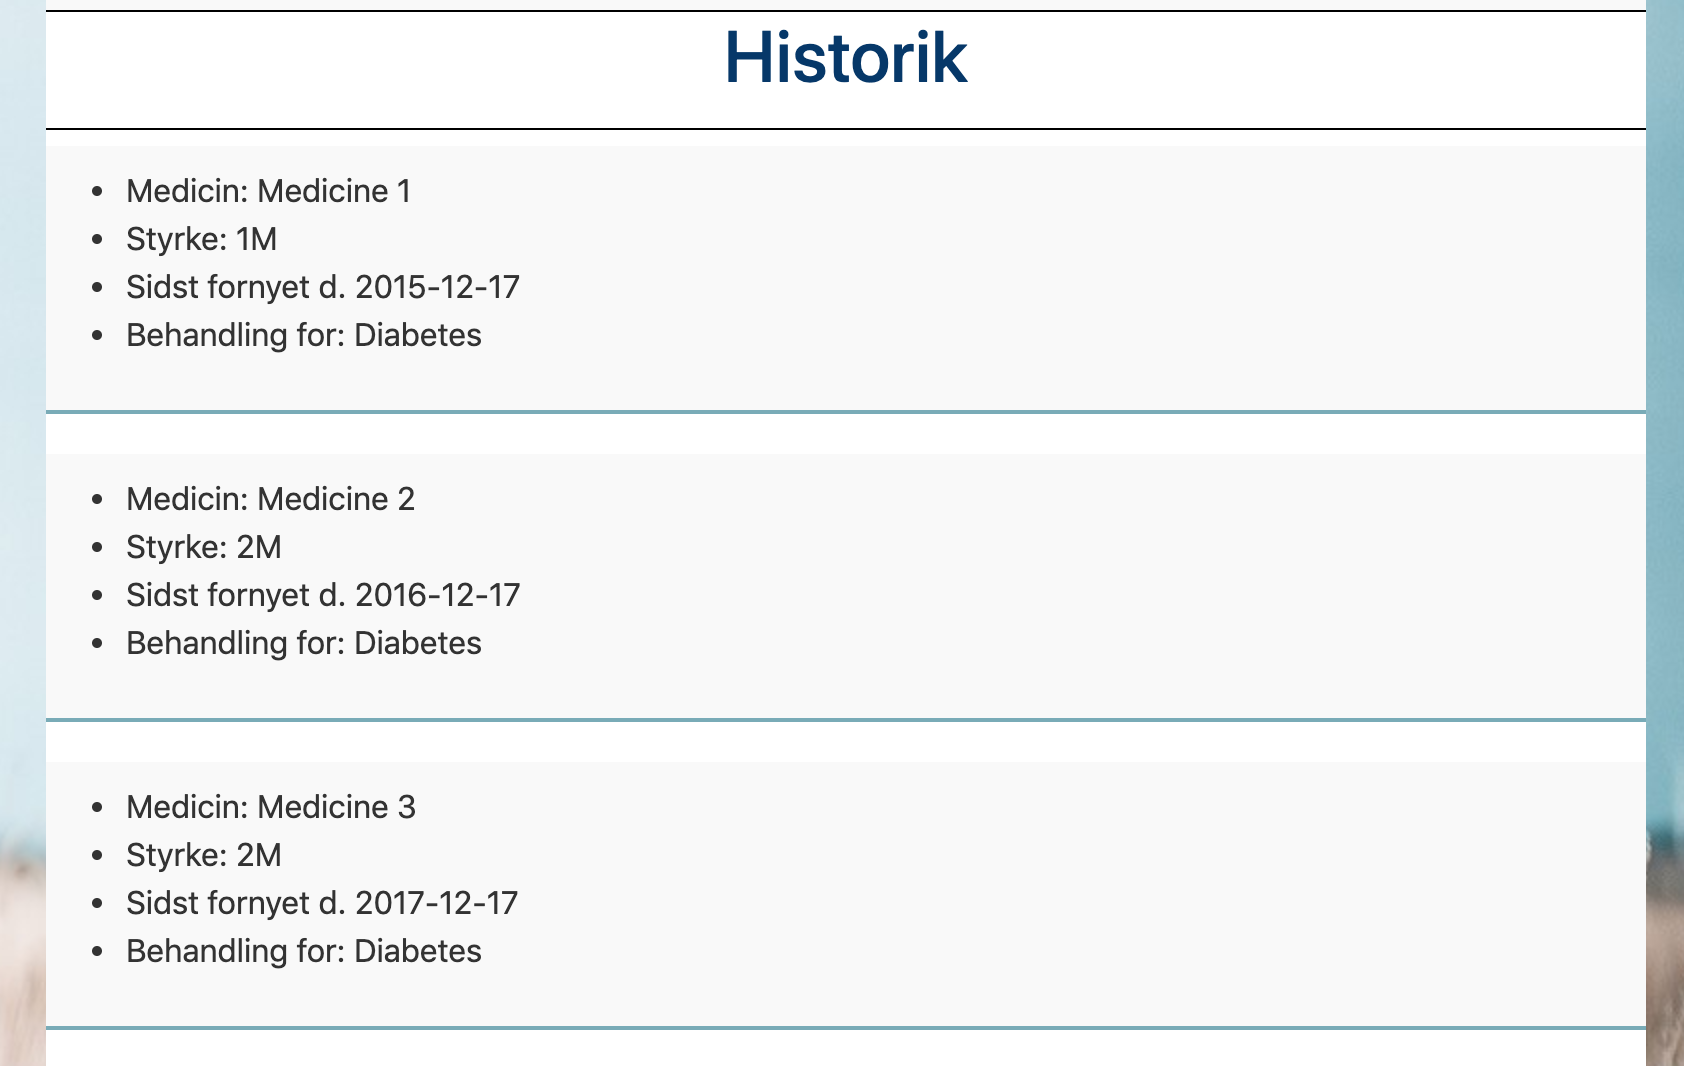
\includegraphics[width=\linewidth]{Materials/Prototype/Historik}
	\caption{Historik for en bruger}
\end{figure}

Vores prototype består hovedsagligt af tre funktionaliteter: \textit{Receptfornyelse, Historik} og \textit{Sundhedsdata}. Under \textit{Historik} er det muligt at se alle ens recepter og tidligere recepter, samt information omkring hvornår recepten blev udskrevet, hvornår den udløb og hvilken medicin der blev udskrevet.\\
Under \textit{Receptfornyelse} kan alle ens aktive recepter ses. Øverst på siden er en processlinje som beskriver hvor langt i 'forløbet' ens medicin er kommet, altså er medicinen først lige bestilt? Har lægen godkendt receptfornyelsen? Kan medicinen afhentes? Denne processlinje understøtter vores vision om at brugeren skal indrages i forløbet, og selv kan se fremskridtene i processen. Nedenunder ses de aktive recepter samt en knap som tillader at fornye recepten. Når brugeren klikker forny ud fra en af sine recepter, så opdateres recepten til ikke længere at være aktiv, og der bliver i stedet lavet en ny recept. I prototypen er de fleste af værdierne i den nye recept hard coded, men dette ville nemt kunne gøres mere realistisk ved at lave om i vores database model.
\begin{figure}[h!]
	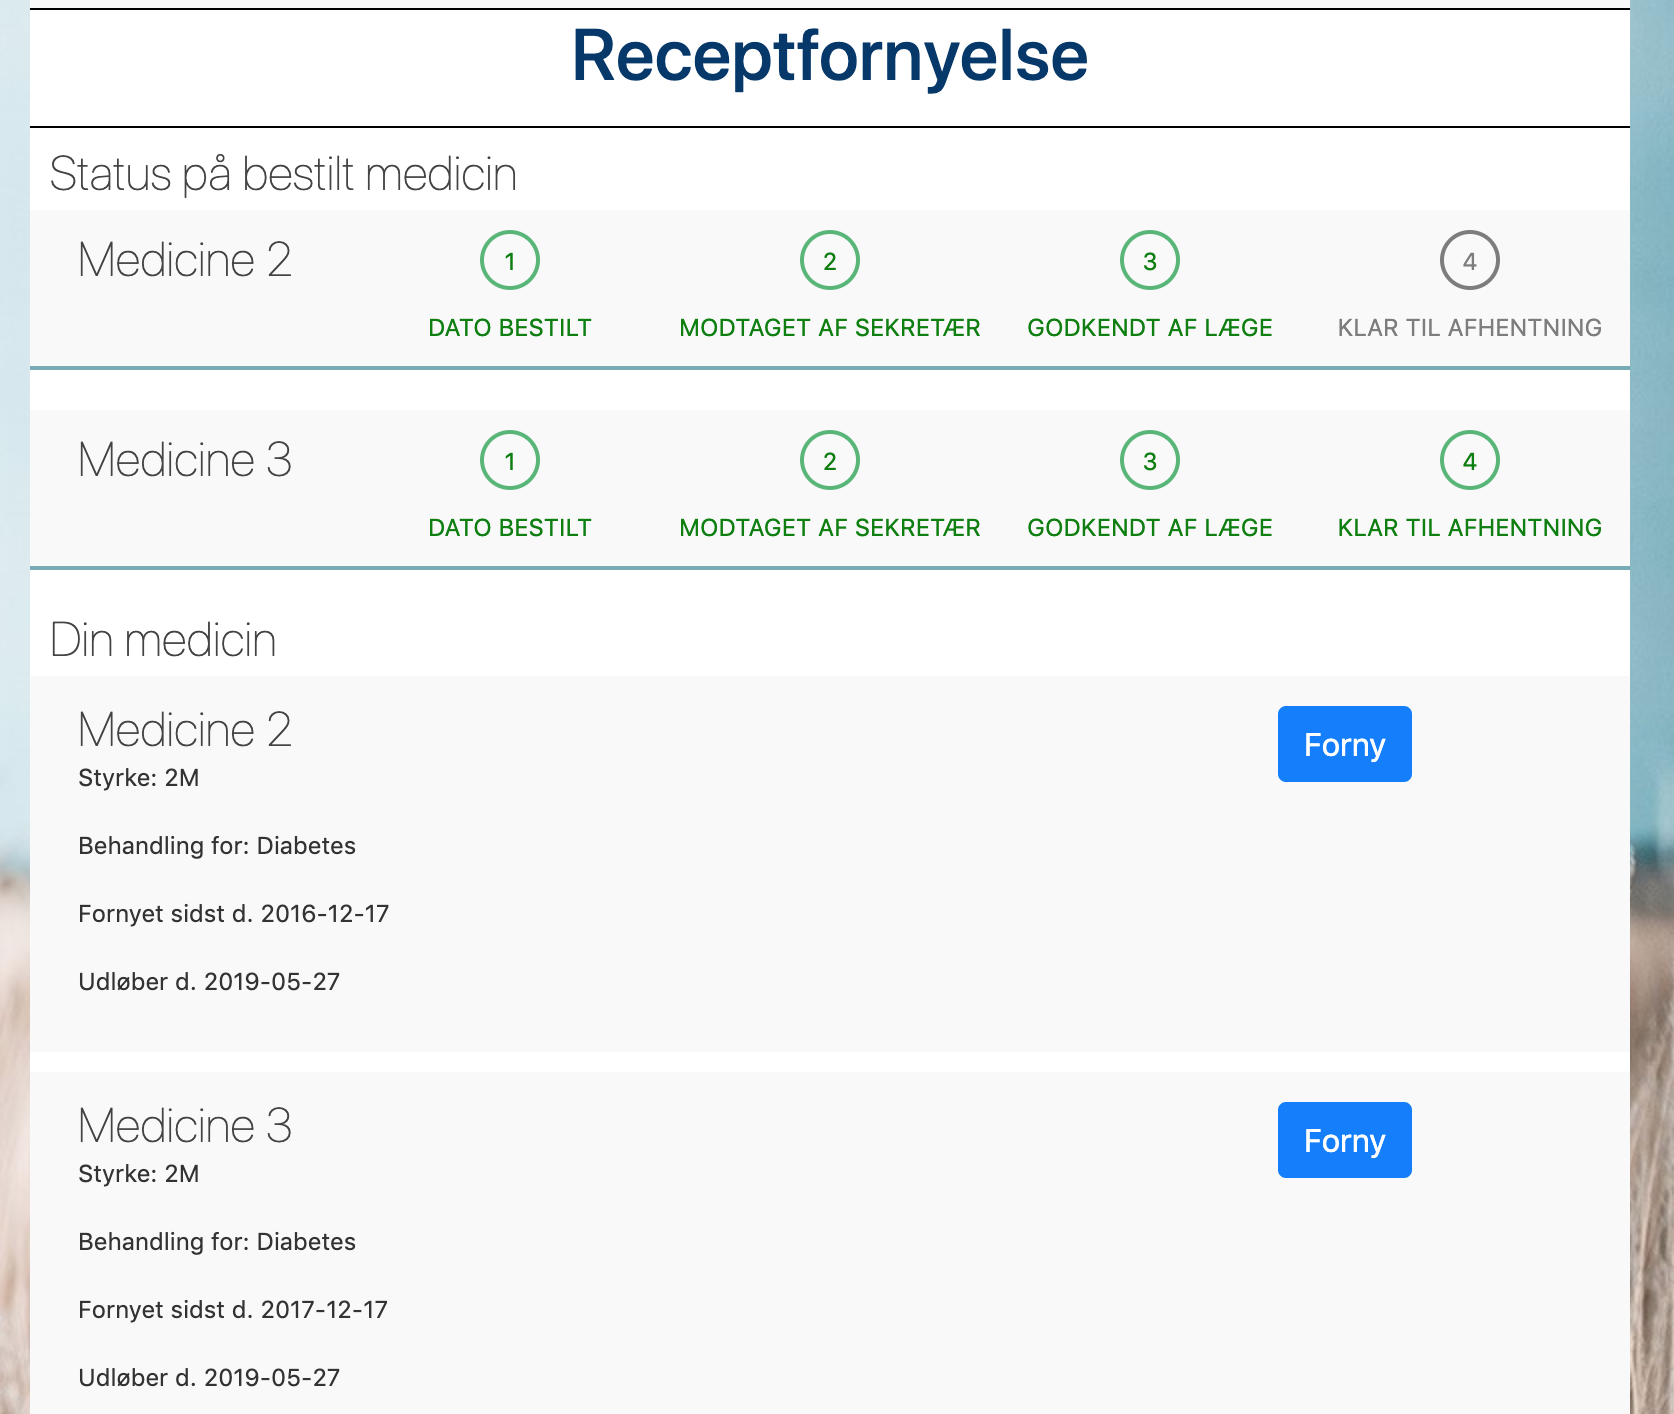
\includegraphics[width=0.49\linewidth]{Materials/Prototype/Receptfornyelse}
	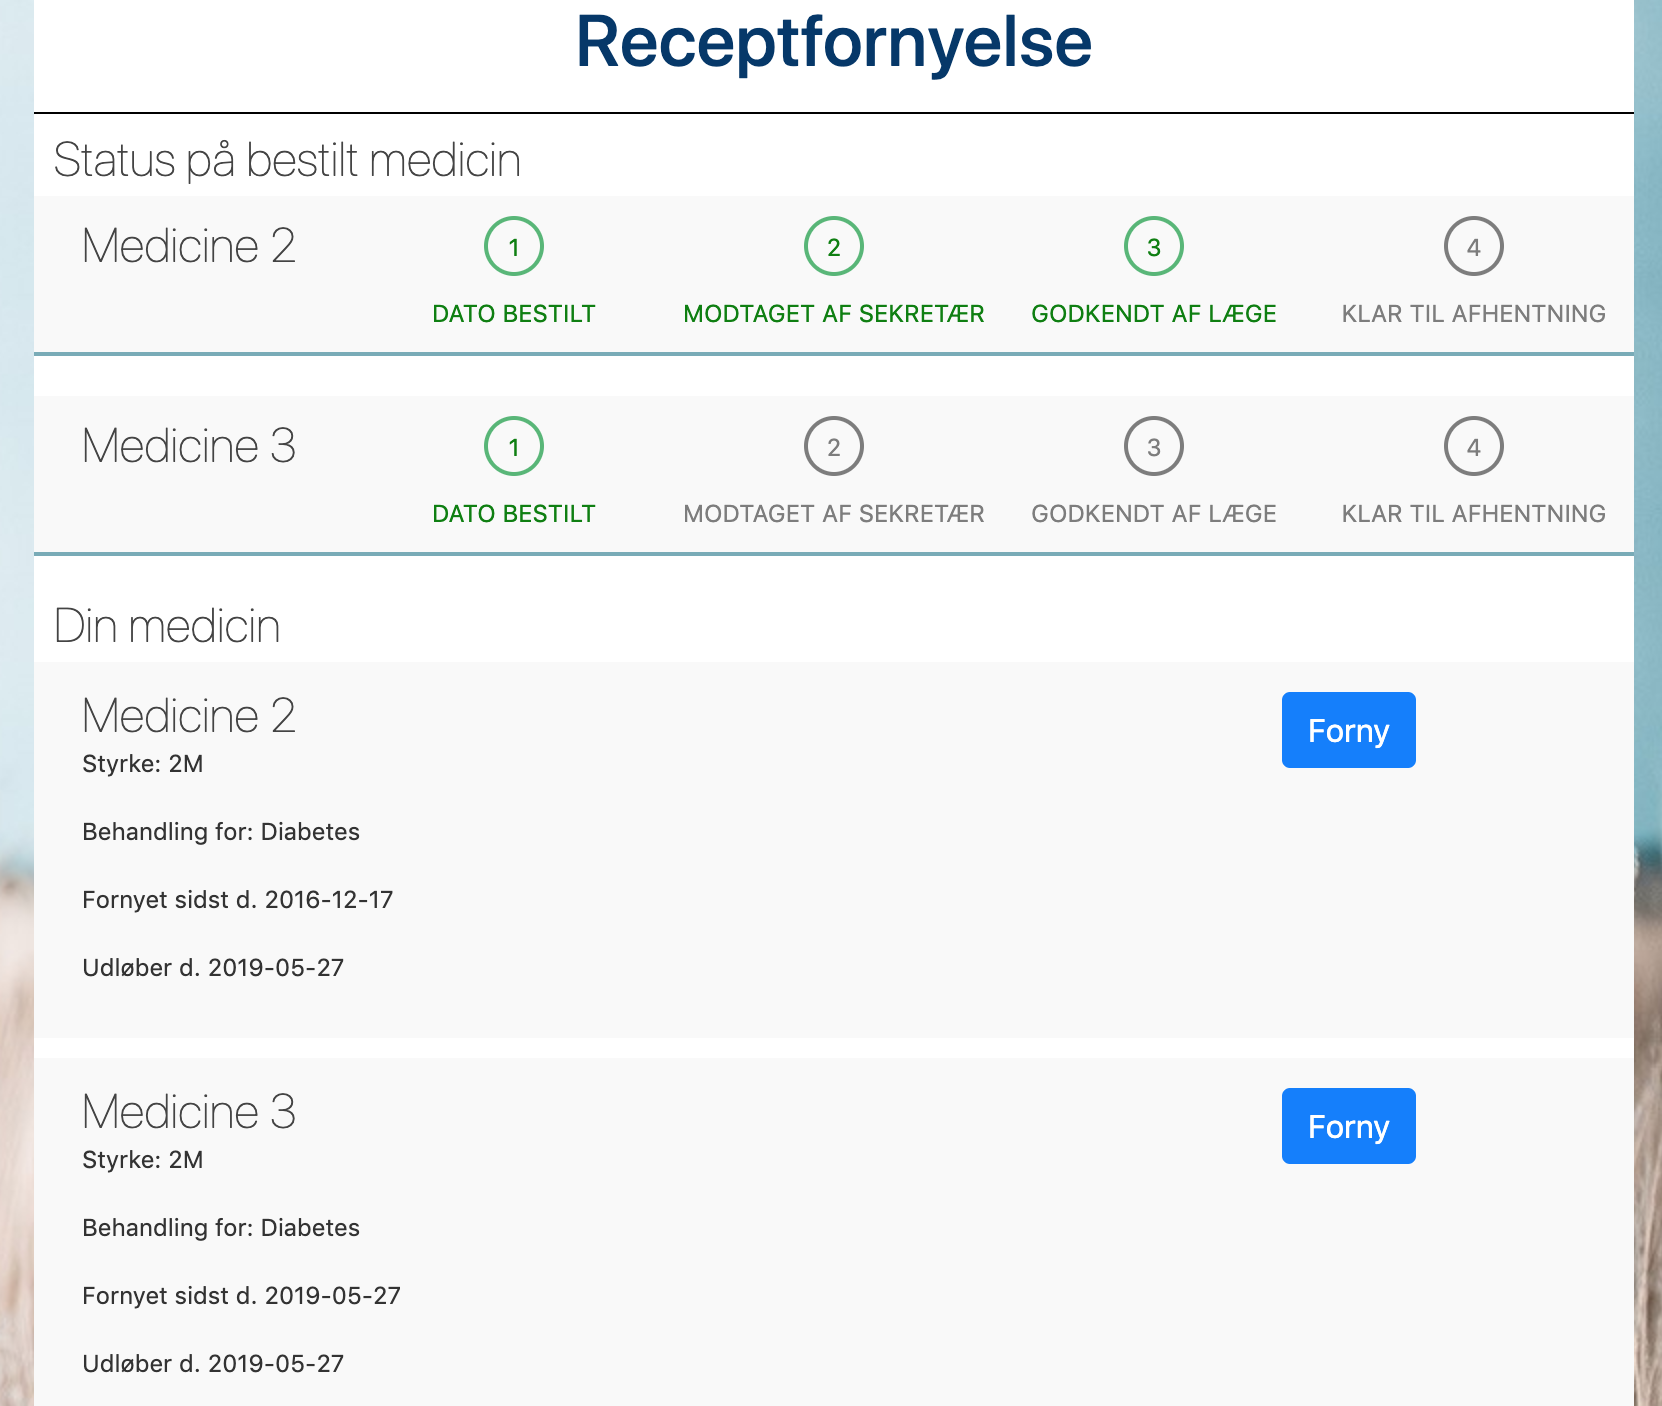
\includegraphics[width=0.49\linewidth]{Materials/Prototype/ReceptfornyelseFornyet}
	\caption{tv. ses recepterne før fornyelse. th. ses recepterne efter 'Medicine 3' fornyelse}
\end{figure}
\todo{Medicin kort?}

%\newpage

\subsection{Known shortcommings}
Der er endnu ikke implementeret business logic til at sørge for, at recepten kun kan fornys, når den er ved at udløbe, og den kan derfor fornys så ofte, det ønskes.\\
Mange værdier er hard-coded, når der indsættes en ny recept gennem receptfornyelsen. Dette ville relativt nemt kunne løses ved at lave om på database-modellen. Da dette er en prototype, hvis formål er at illustrere en mulig løsning, har dette ikke været en prioritet at løse.\\
Flere sider kan tilgås uden at være logget ind, hvilket i de fleste tilfælde bare efterlader en blank side. Dette har ikke været en prioritet at løse, da hele login delen af prototypen ville skulle udskiftes med NemID.\\


\section{Anbefalinger og prioriteringer}
I denne forundersøgelsesrapport har vi beskrevet følgende:
\begin{itemize}
	\item Visioner om den samlede forandring
	\item Fordele og ulemper ved implementering
	\item Startegi og plan for implementering
	\item Prototype for receptfornyelse
\end{itemize}
Det er hensigten, at prototypen skal kunne give et indblik i design visionen for receptfornyelsesmodulet og ville kunne bruges til at afprøve, hvordan arbejdsgangen vil være mellem interessenterne.\\
Prototypen kan være en hjælp til softwareudviklerne til at få en bedre forståelse af, hvordan receptfornyelsesmodulet skal udvikles. Derudover er intentionen, at en udviklet prototype ville hjælpe med til at finde diverse problemer, som vores implementation skaber, men som ikke fra starten er åbenlyse. \\\\
Samlet set er rapporten ment som et beslutningsgrundlag for Region Sjælland om igangsætning af udvikling og implementering af de forslåede ændringer til MinSP.

\section{Bilag 1: User stories}
%User stories:
%
%Independece
%Der må ikke være afhægihed mellem histrierne
%Afhægihed mellem historierne: giver planlægningens / prioterings problemer
%
%Negotiable
%Kort beskrivelse af funktionalitet
%Detajerne omkring hvordan det skal skal ikke være med - det er til forhandling.
%De er husker om hvad vi skal have med.
%Tilføj kort 'Note', hvis der detajer/overvejelser der er vigtige at have med.
%
%Vauluable to Purchasers or Users
%Skal skrives så man ser fordel for brugernes synspunkt - ikke kundens /programmørens
%Brugernes antagelser om interfacet skal ikke med
%Teknologi antagelse skal ikke med
%
%Estimatable
%De skal kunne estimeres dvs. vurdere hvad det vil koste at udvikle for at udvikle det.
%User stories skal bruges i konsekvens analysen når man skal estimere omkostninger.
%
%Small
%Det skal være konkret. Feks det må ikke være ' en bruger skal kunne bestille en rejse ' (epic) det skal være splittet op:
%          ' en bruger skal kunne kontakte rejse bureauet '
%
%Test
%Man skal kunne skrive test ud fra dem
\subsection{User Stories}
\subsubsection{Current User Stories} % Current User stories er for hver af de relevante aktøre i Domænet
Current User Stories er udarbejdet ud fra ER diagrammet over domænet for MinSP. \footnote{Bilag 4} 
\subsubsection*{Som patient:}
\begin{itemize}
\item kan jeg se min Journal. Note: Journal har journalnotater. 
\item kan jeg se min diagnose-oversigt.
\item kan jeg se min målings-oversigt.
\item kan jeg modtage beskeder og se dem i min Indbakke.
\item kan jeg sende beskeder og se dem i min Udbakke.
\item kan jeg modtage påmindelser.
\item kan jeg se mine aftaler. 
\item kan jeg se mine prøvesvar.
\item kan jeg udfylde et spørgeskema.
\item kan jeg give en fuldmagt. 
\item har jeg kontakt med sundhedsfaglige personer. 
\item som patient, kan jeg så se, hvem der har været logget på min journal.
\end{itemize}
\subsubsection*{Som sundhedsfaglig person:}
\begin{itemize}
\item har jeg kontaktansvar for flere patienter.
\item skal jeg kunne logge på og skrive notater i patienters journal.
\end{itemize}
\subsubsection{Furture User Stories}
Furture user stories er udarbejdet ud fra vores bruger-undersøgelser.
\subsubsection*{Som diabetes patient:}
\textbf{Fra interview}\\
\begin{itemize}
\item CUKaren: Ønsker jeg at kunne læse information omkring diabetes på MinSP, så jeg ikke skal søge flere steder. \\
Note: information kan være om diabetes og om kost.
\item CUJulia: Ønsker jeg, at oplysninger om mine diagnoser er adskilte, for at opnå en mere personlig MinSP. 
\item CUKaren: Ønsker jeg, at jeg direkte ledes det rigtig sted hen i menuen og ikke af omveje, så jeg ikke leder forgæves.\\ 
Note: Brugervenlighed f.eks. i forhold til receptfornyelse.
\item CUErnest: Ønsker jeg at modtage reminders om kost og motion for at blive motiveret.
\item CUJannie: Ønsker jeg at kunne forstå min prøvesvar, så jeg ved, hvad de betyder. \\
Note: En dansk forklaring af resultatet, hvilket hospital, prøven er taget på og til hvilken diagnose. 
\item CUErnest: Ønsker jeg at kunne se, hvor indhold i min journal stammer fra, så jeg bedre kan overskue det.
\item CUPeter: Ønsker jeg påmindelse om receptfornyelse, konsultation mv., så jeg ikke skal huske på det selv.\\ 
Note: kunne vælge mellem e-boks, email, sms.
\item CUKaren: Ønsker jeg at kunne tilgå et diskussionsforum for patienter for at møde ligesindede.
\end{itemize}
\textbf{Fra spørgeskema-undersøgelse}\\
\begin{itemize}
\item CU1: Ønsker jeg mulighed for at forny min recept gennem MinSP, så jeg kun skal ind et sted og ikke skal vente i telefonen.
\end{itemize}
%
% Ydligere funktioner nogen i gruppen har snakket om /forslået:
% - Skype / videosamtale med sundhespersonale / læge
% - Nyt udstyr der måler blodsukker og sender det til MinSP => giver en graf over det (der kan f.eks. laves en Mock-up),
% -

\newpage
\section{Bilag 2: MoSCoW Prioritering}
%MoSCoW Prioritering
\subsection{MoSCoW Prioritering}
\subsubsection{Must have}
\subsubsection{Should have}
%
% ? - Anders Lassen: "Læring og videnscenter. Der er allerede patienthåndbogen Jeg tror det er out-of-scope":
- CUKaren: Jeg ønsker at kunne læse information omkring diabetes på MinSP. Note: information kan være om diabetes og om kost.\\ % Dyr at vedligeholde af sundhedspersonalet. Muligevis laves med link til patienthåndbogen.
- CUJannie: Jeg ønsker nemt at kunne forstå min prøvesvar. Note: En dansk forklaring af resultatet: der indeholder hvilken hospital prøven er taget på, i forhold til hvilken diagnose og hvorfor denne specifik prøve er taget / hvad den siger noget om. Med evt. en graf over udviklingen af prøvesvar f.eks. over blodsukker.\\
- CUKaren: Jeg ønsker at jeg direkte ledes det rigtig sted hen i menuen og ikke af omveje. Note: Brugervenlighed - i forhold til receptfornyelse samt booking af aftaler.\\ 
- CUJulia: Jeg ønsker at oplysninger om mine diagnoser er adskilte. Note: for at opnå en mere personlig MinSP.\\
\subsubsection{Could have}
- CUErnest: Jeg ønsker at modtage reminders om kost og motion. Note: Motivation. \\
- CUErnest: Jeg ønsker at kunne se hvor indhold i min journal stammer fra.\\
- CUPeter: Jeg ønsker påmindelse om receptfornyelse. Note: kunne vælge mellem e-boks, email, sms.\\
\subsubsection{Won't have}
- CUKaren: Jeg ønsker at kunne tilgå et diskussionsforum for patienter.\\ % Hvis det er lægen der skal svare på spørgsmål bliver det dyrt.
\section{Bilag 3: Diagnostiske og Virtuelle kort}
\begin{figure}[H]
	\centering
	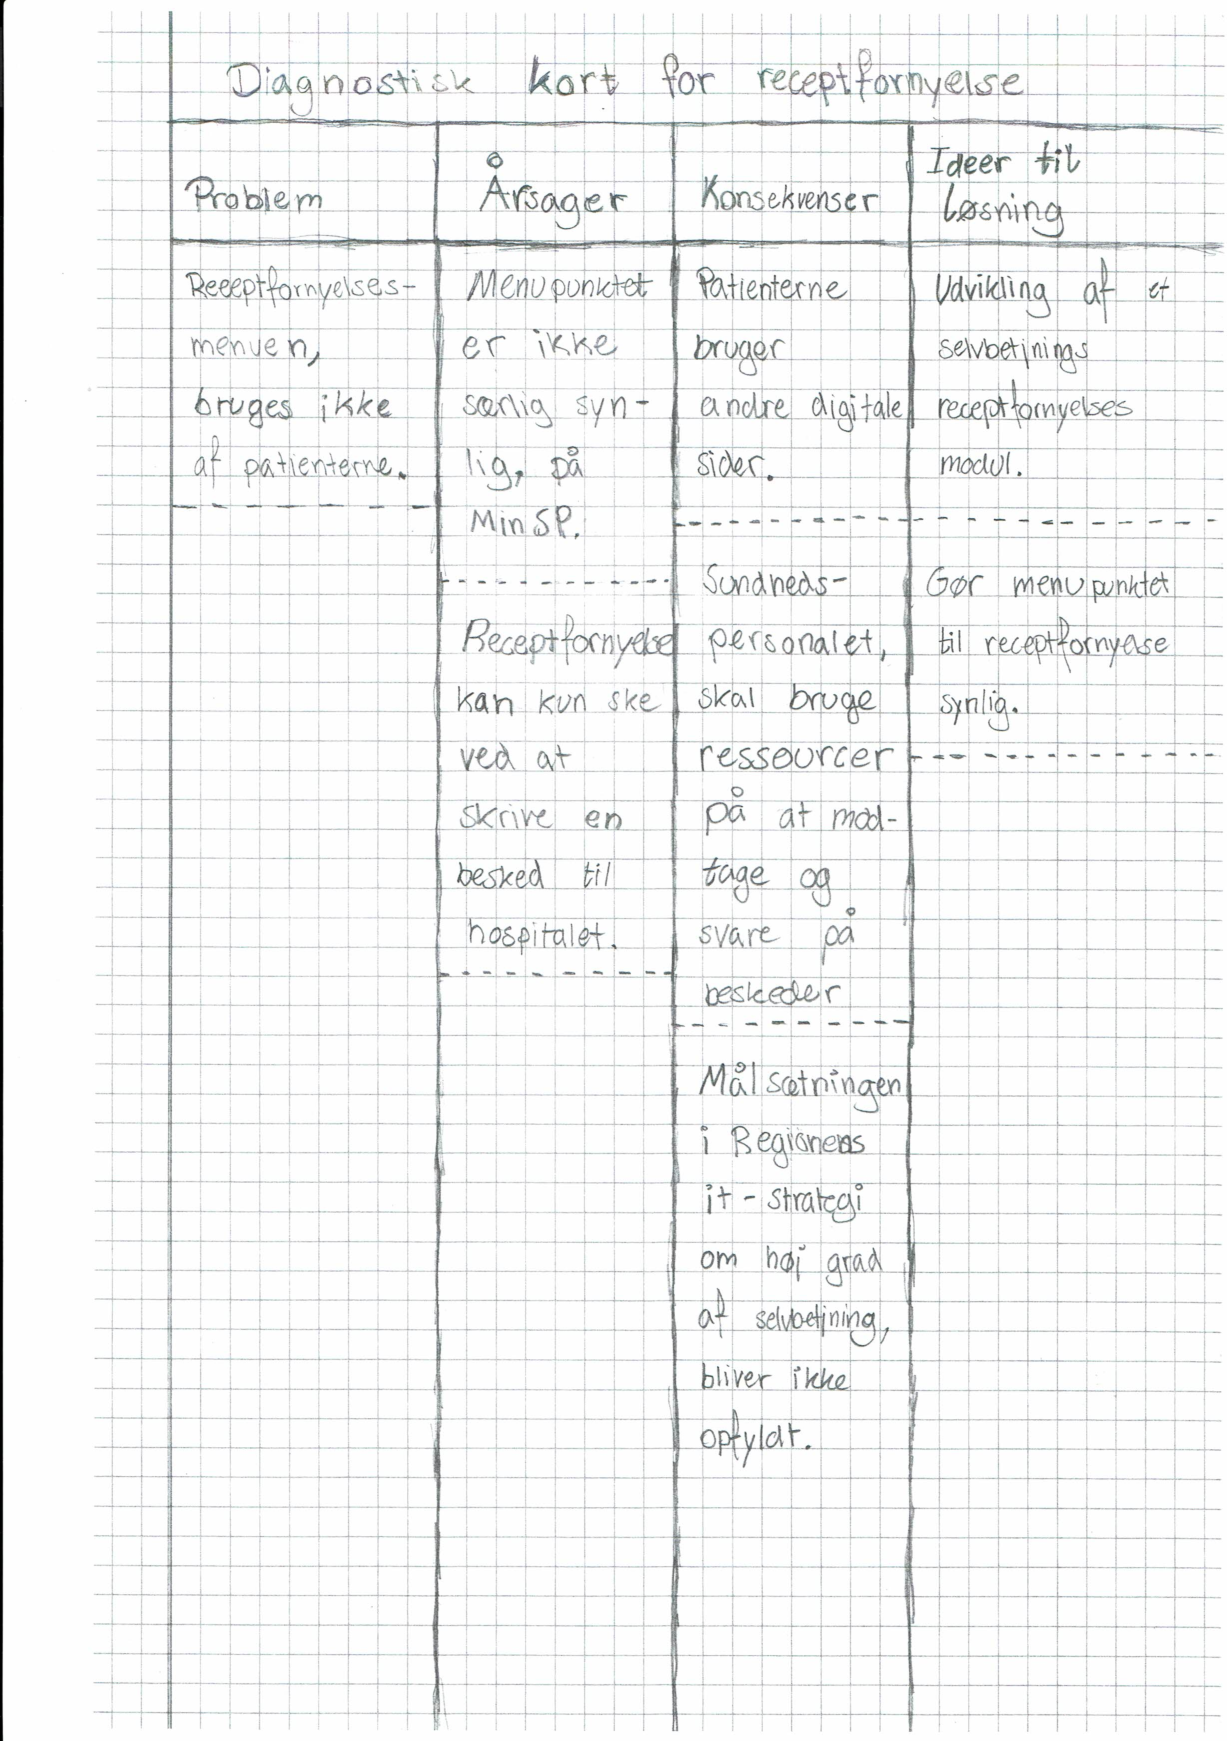
\includegraphics[angle=0, height=0.9\textheight]{Materials/DV_Kort1.pdf}
	%\caption{Mock-up for modulet 'Information om dine diagnoser': Undermenu}
	\label{fig:DVkort1}
\end{figure}
\begin{figure}[H]
	\centering
	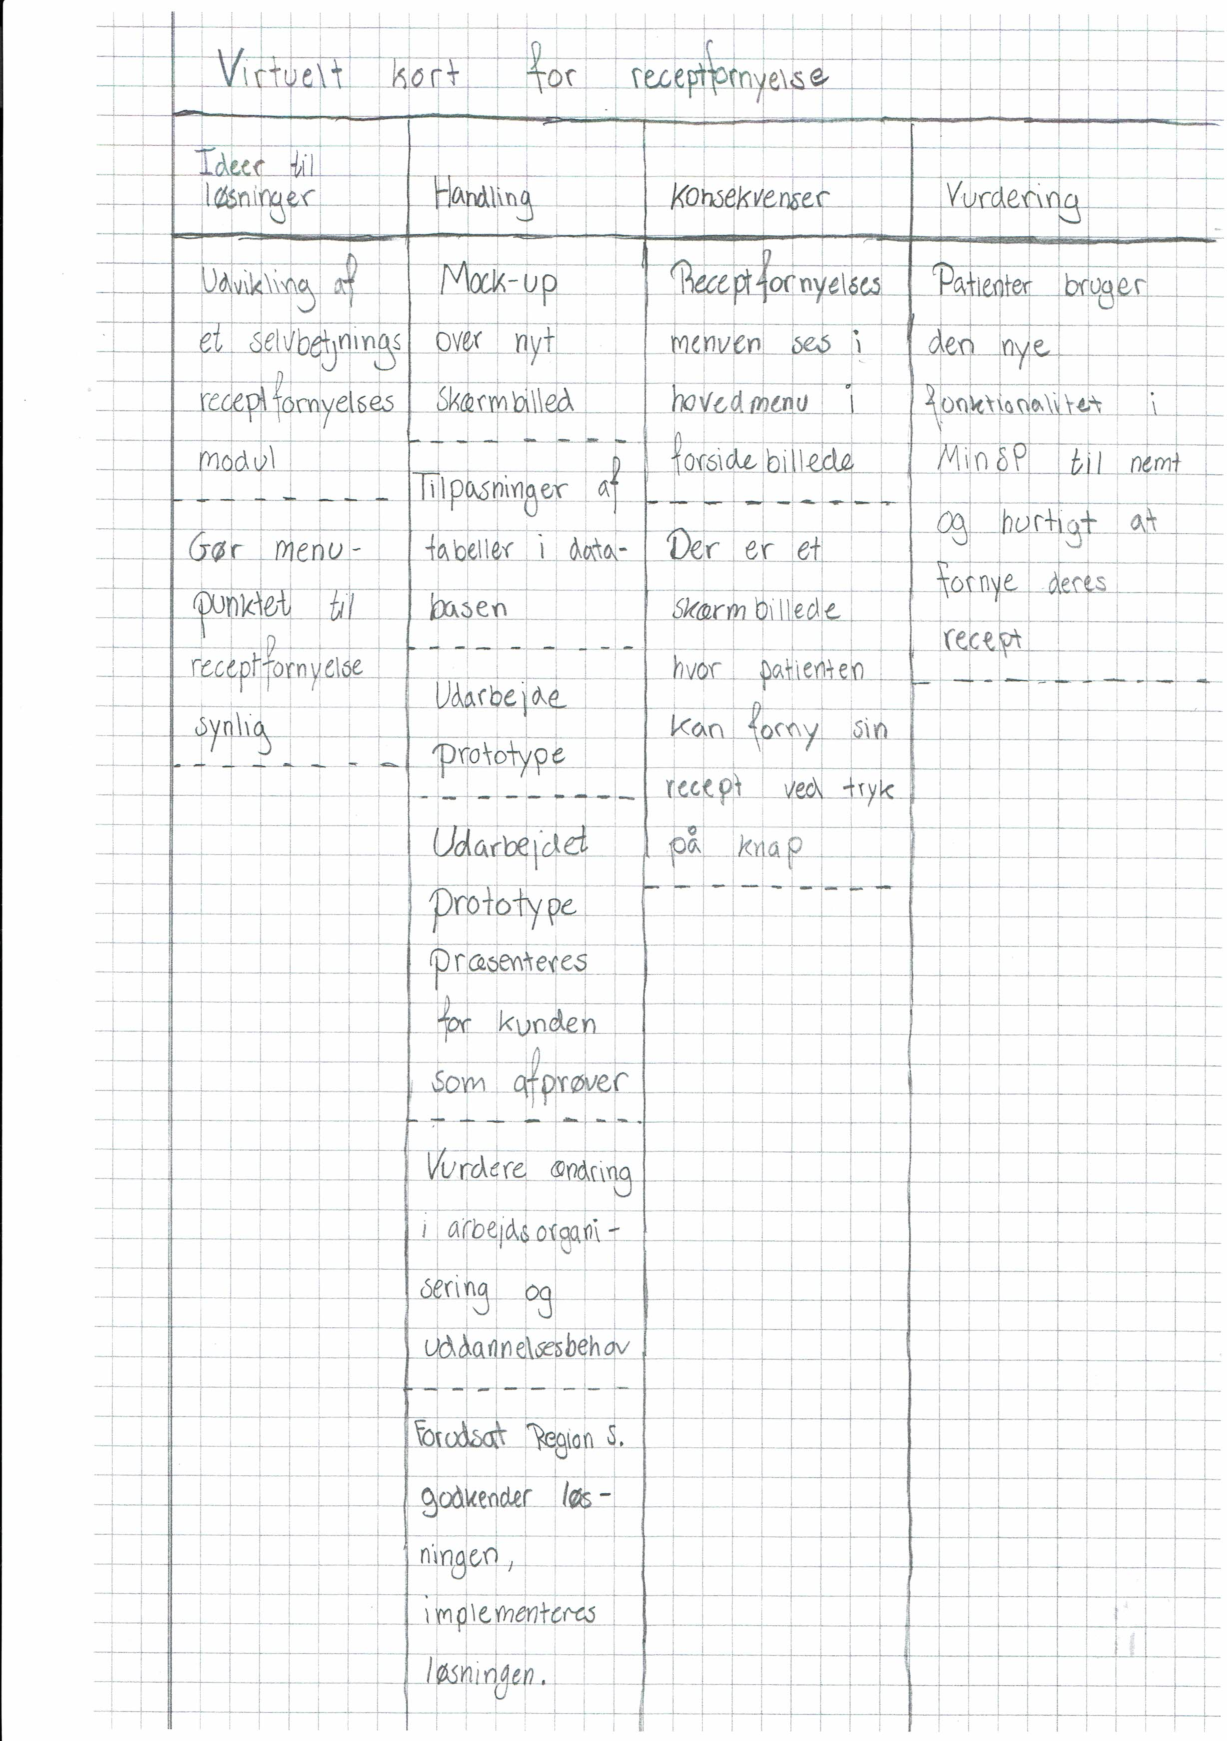
\includegraphics[angle=0, height=0.9\textheight]{Materials/DV_Kort2.pdf}
	%\caption{Mock-up for modulet 'Information om dine diagnoser': Undermenu}
	\label{fig:DVkort2}
\end{figure}
\begin{figure}[H]
	\centering
	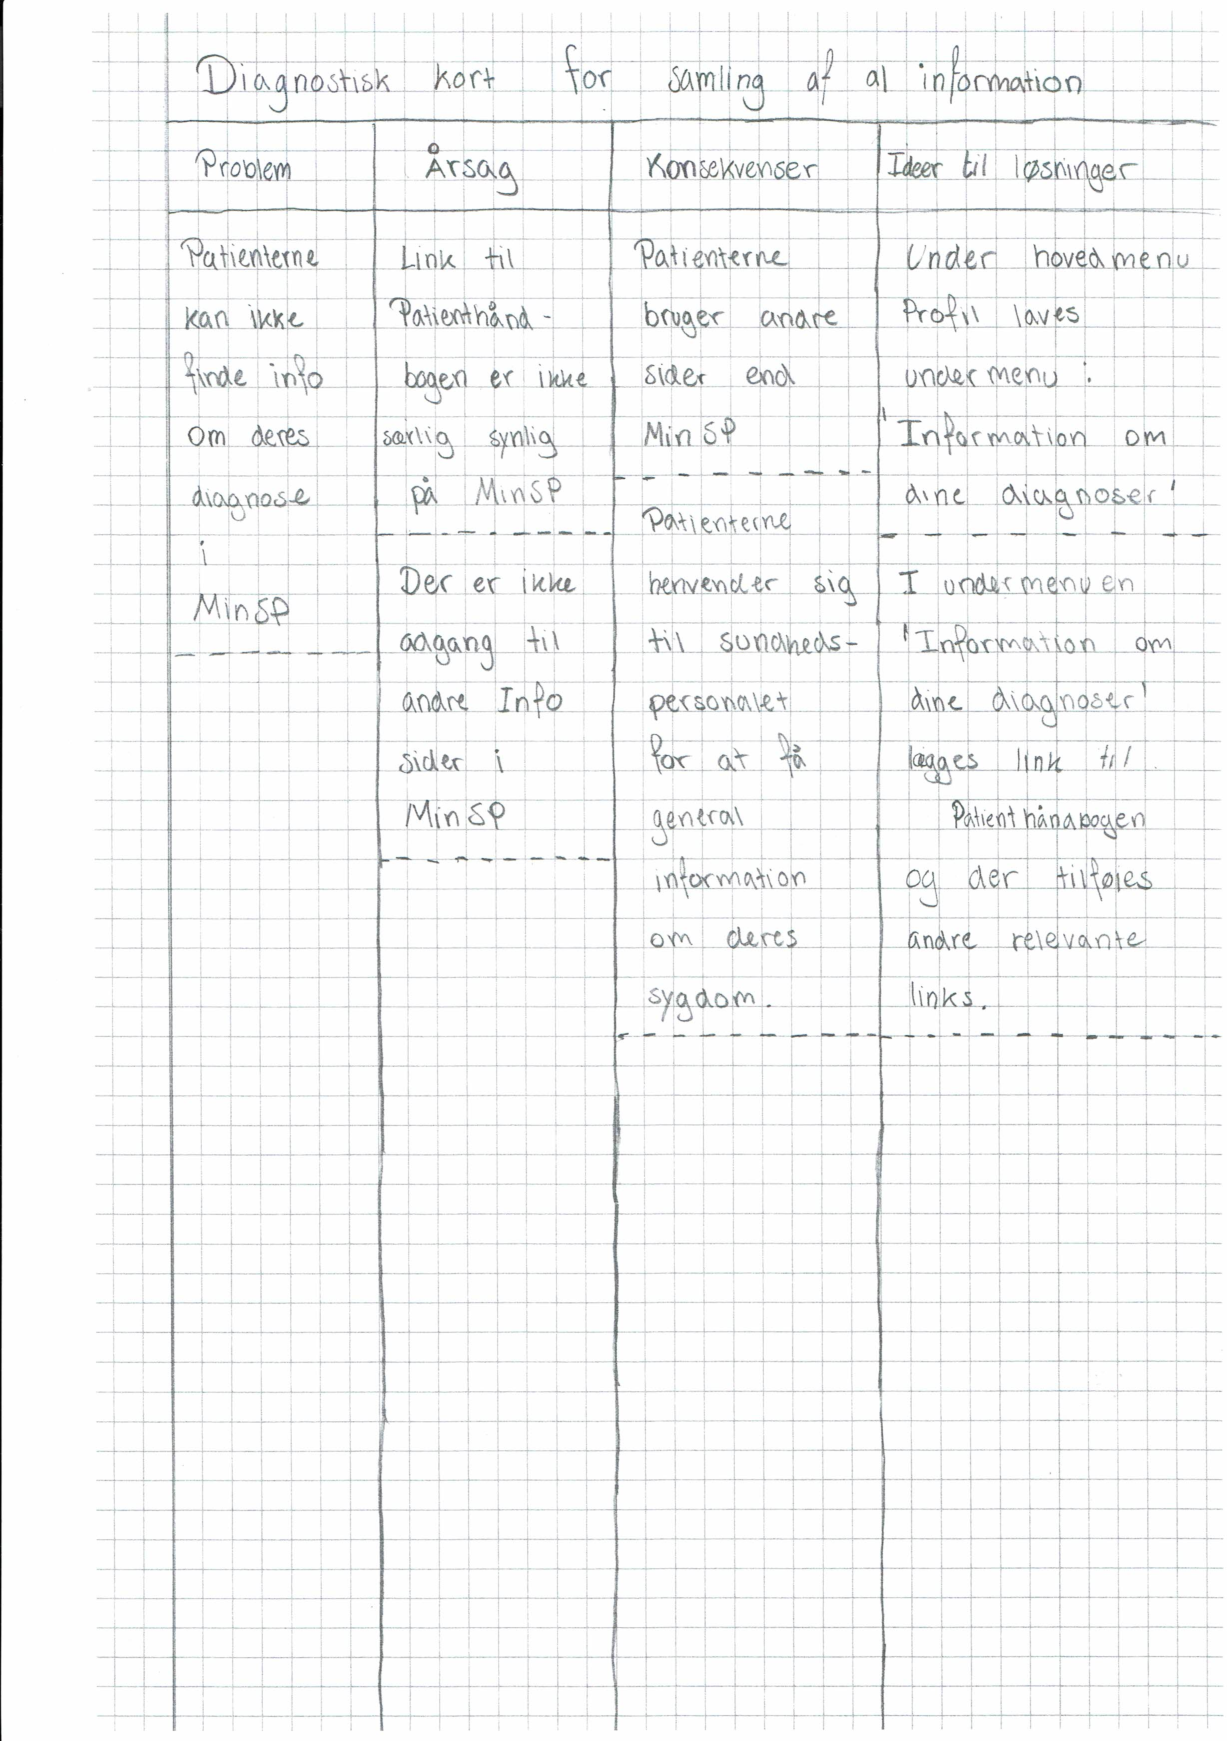
\includegraphics[angle=0, height=0.9\textheight]{Materials/DV_Kort3.pdf}
	%\caption{Mock-up for modulet 'Information om dine diagnoser': Undermenu}
	\label{fig:DVkort3}
\end{figure}
\begin{figure}[H]
	\centering
	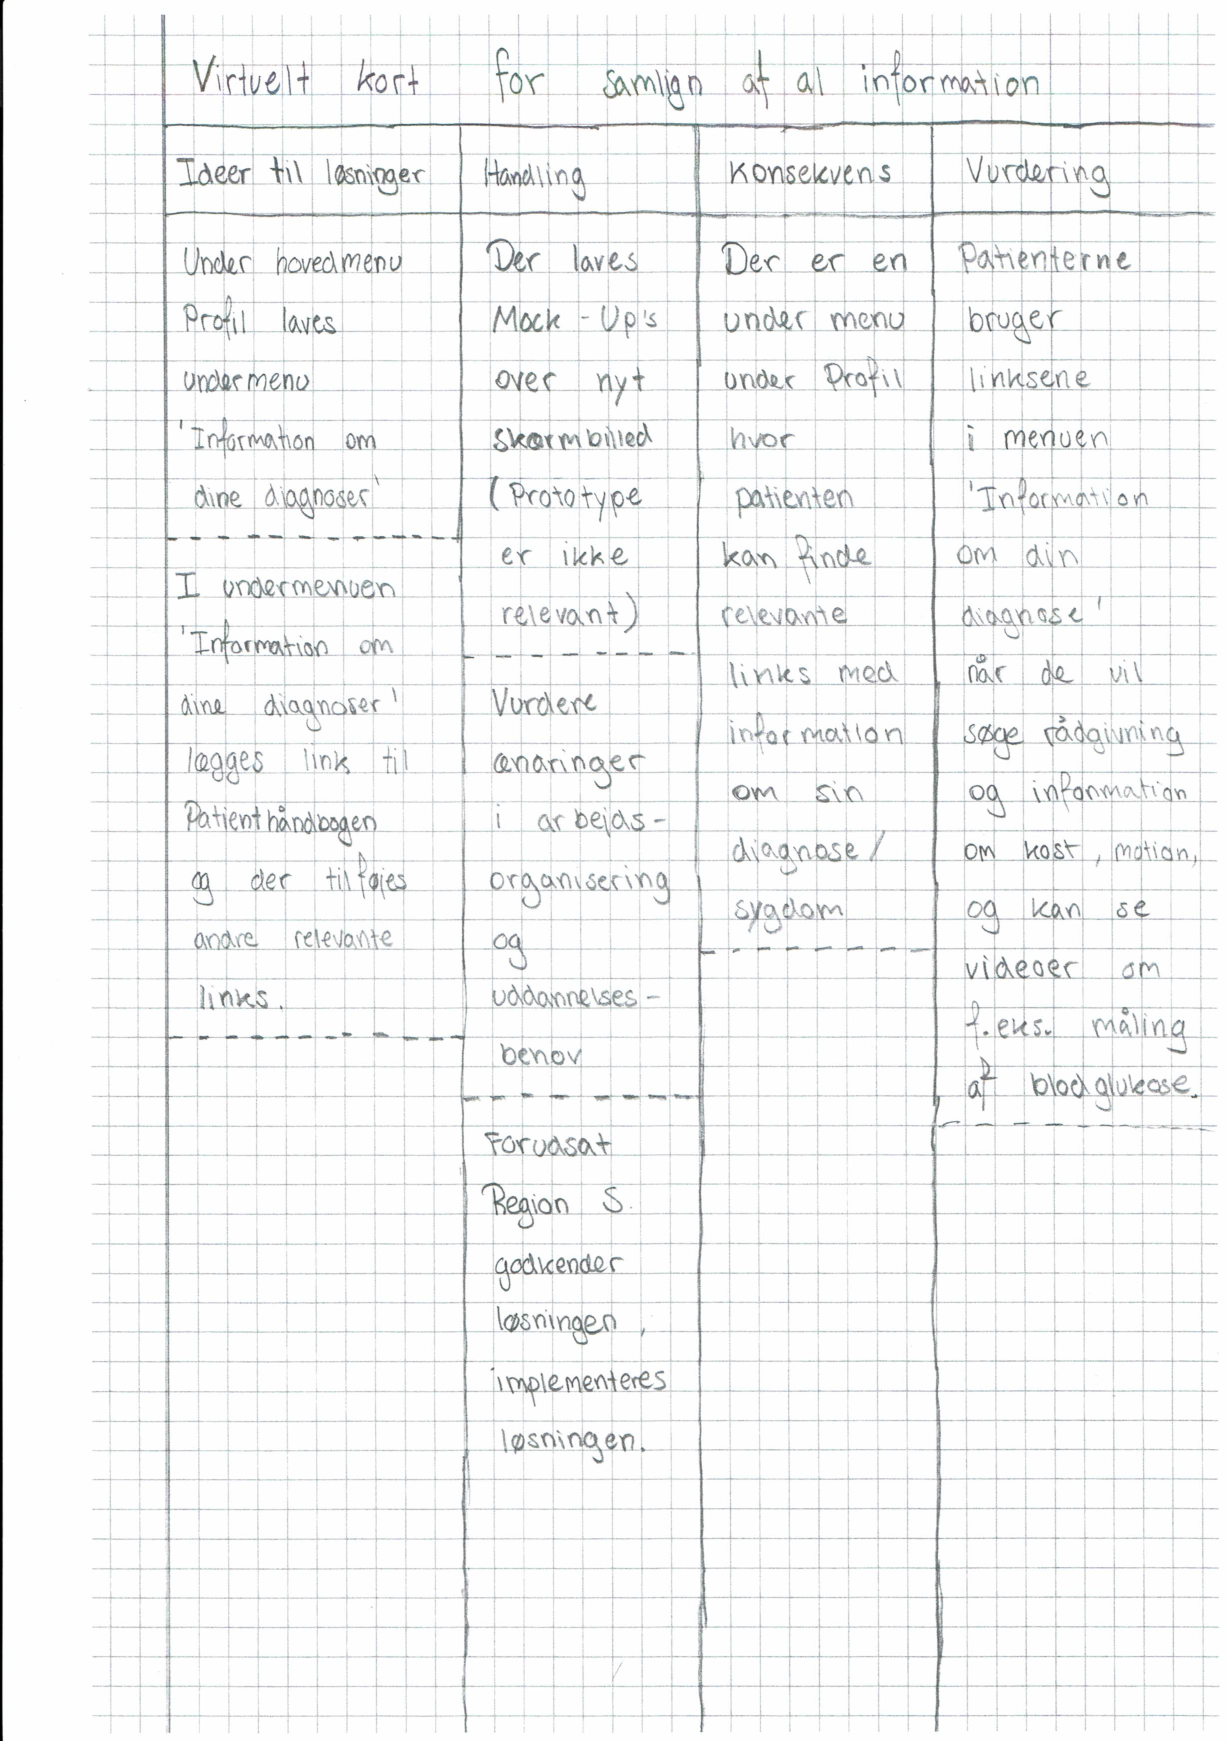
\includegraphics[angle=0, height=0.9\textheight]{Materials/DV_Kort4.pdf}
	%\caption{Mock-up for modulet 'Information om dine diagnoser': Undermenu}
	\label{fig:DVkort4}
\end{figure}
\begin{figure}[H]
	\centering
	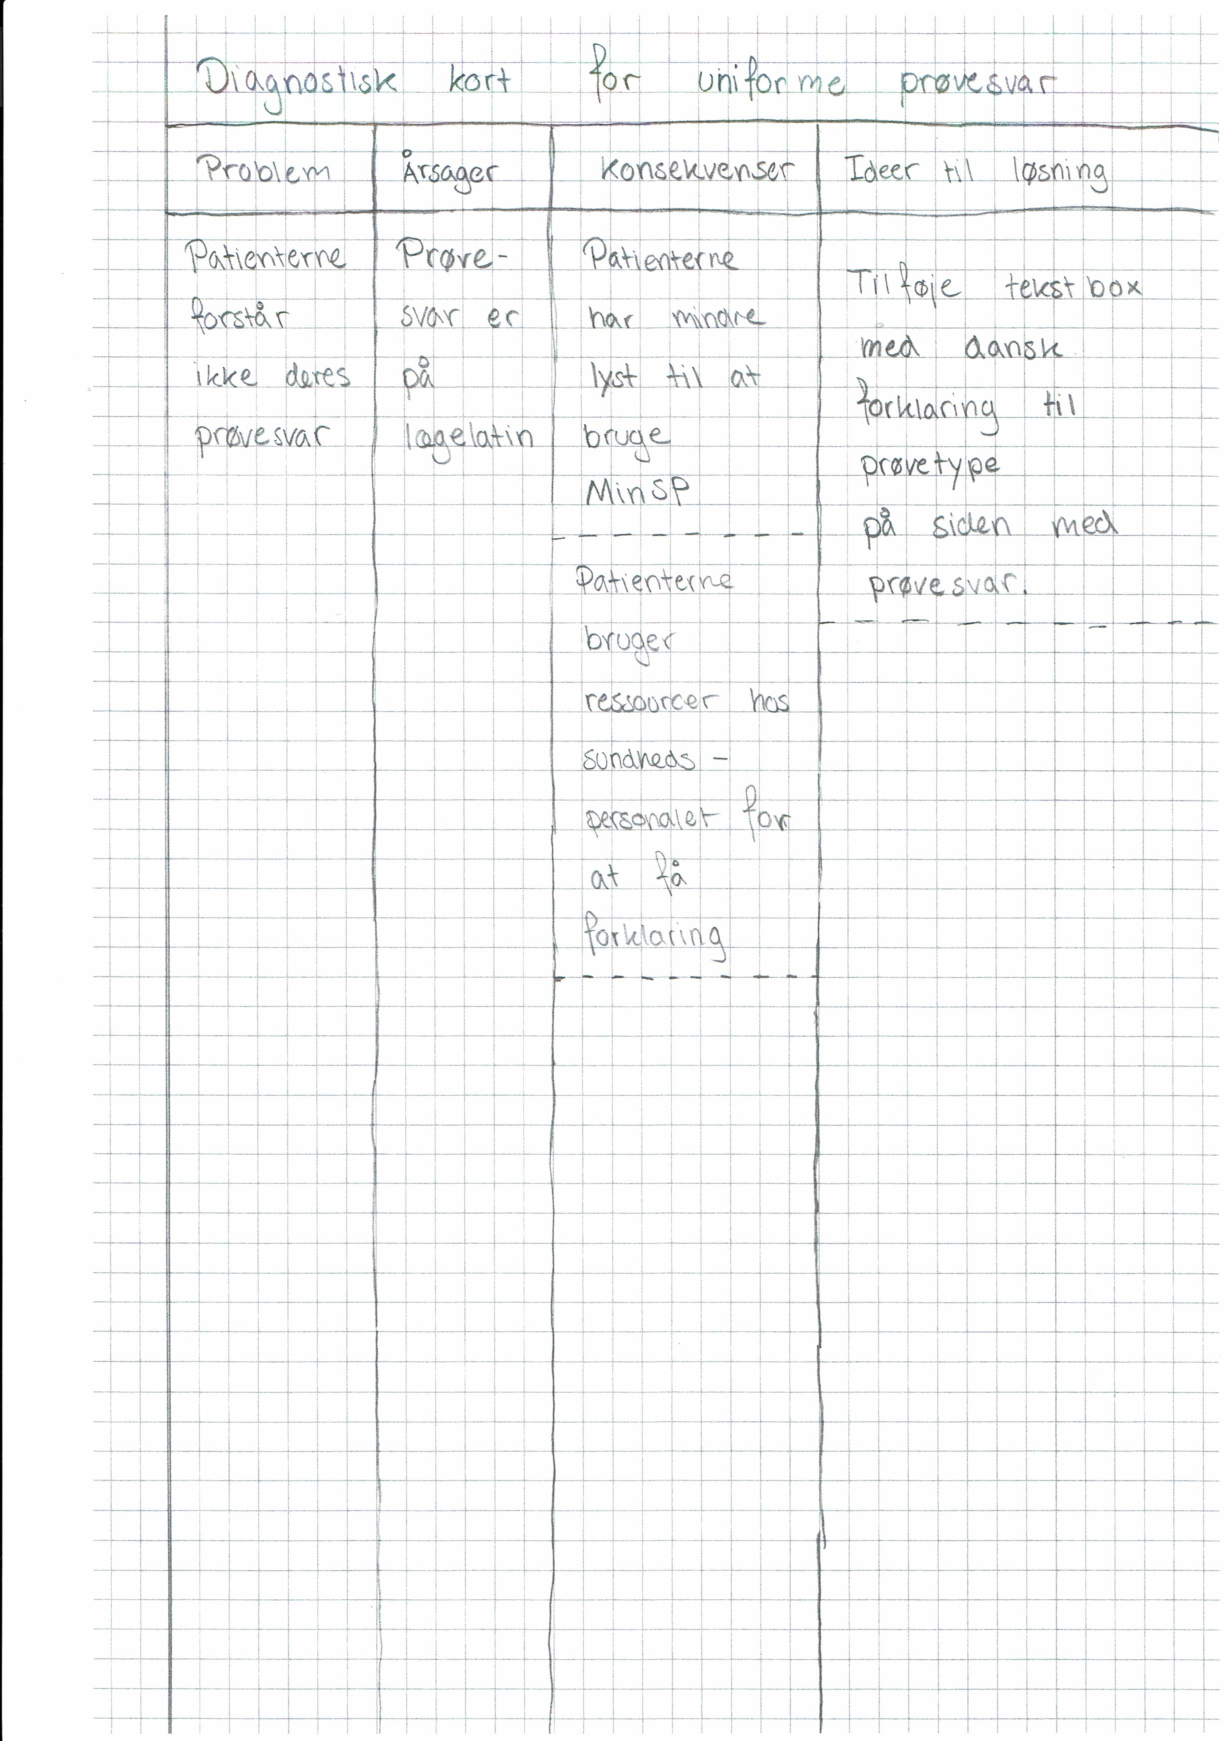
\includegraphics[angle=0, height=0.9\textheight]{Materials/DV_Kort5.pdf}
	%\caption{Mock-up for modulet 'Information om dine diagnoser': Undermenu}
	\label{fig:DVkort5}
\end{figure}
\begin{figure}[H]
	\centering
	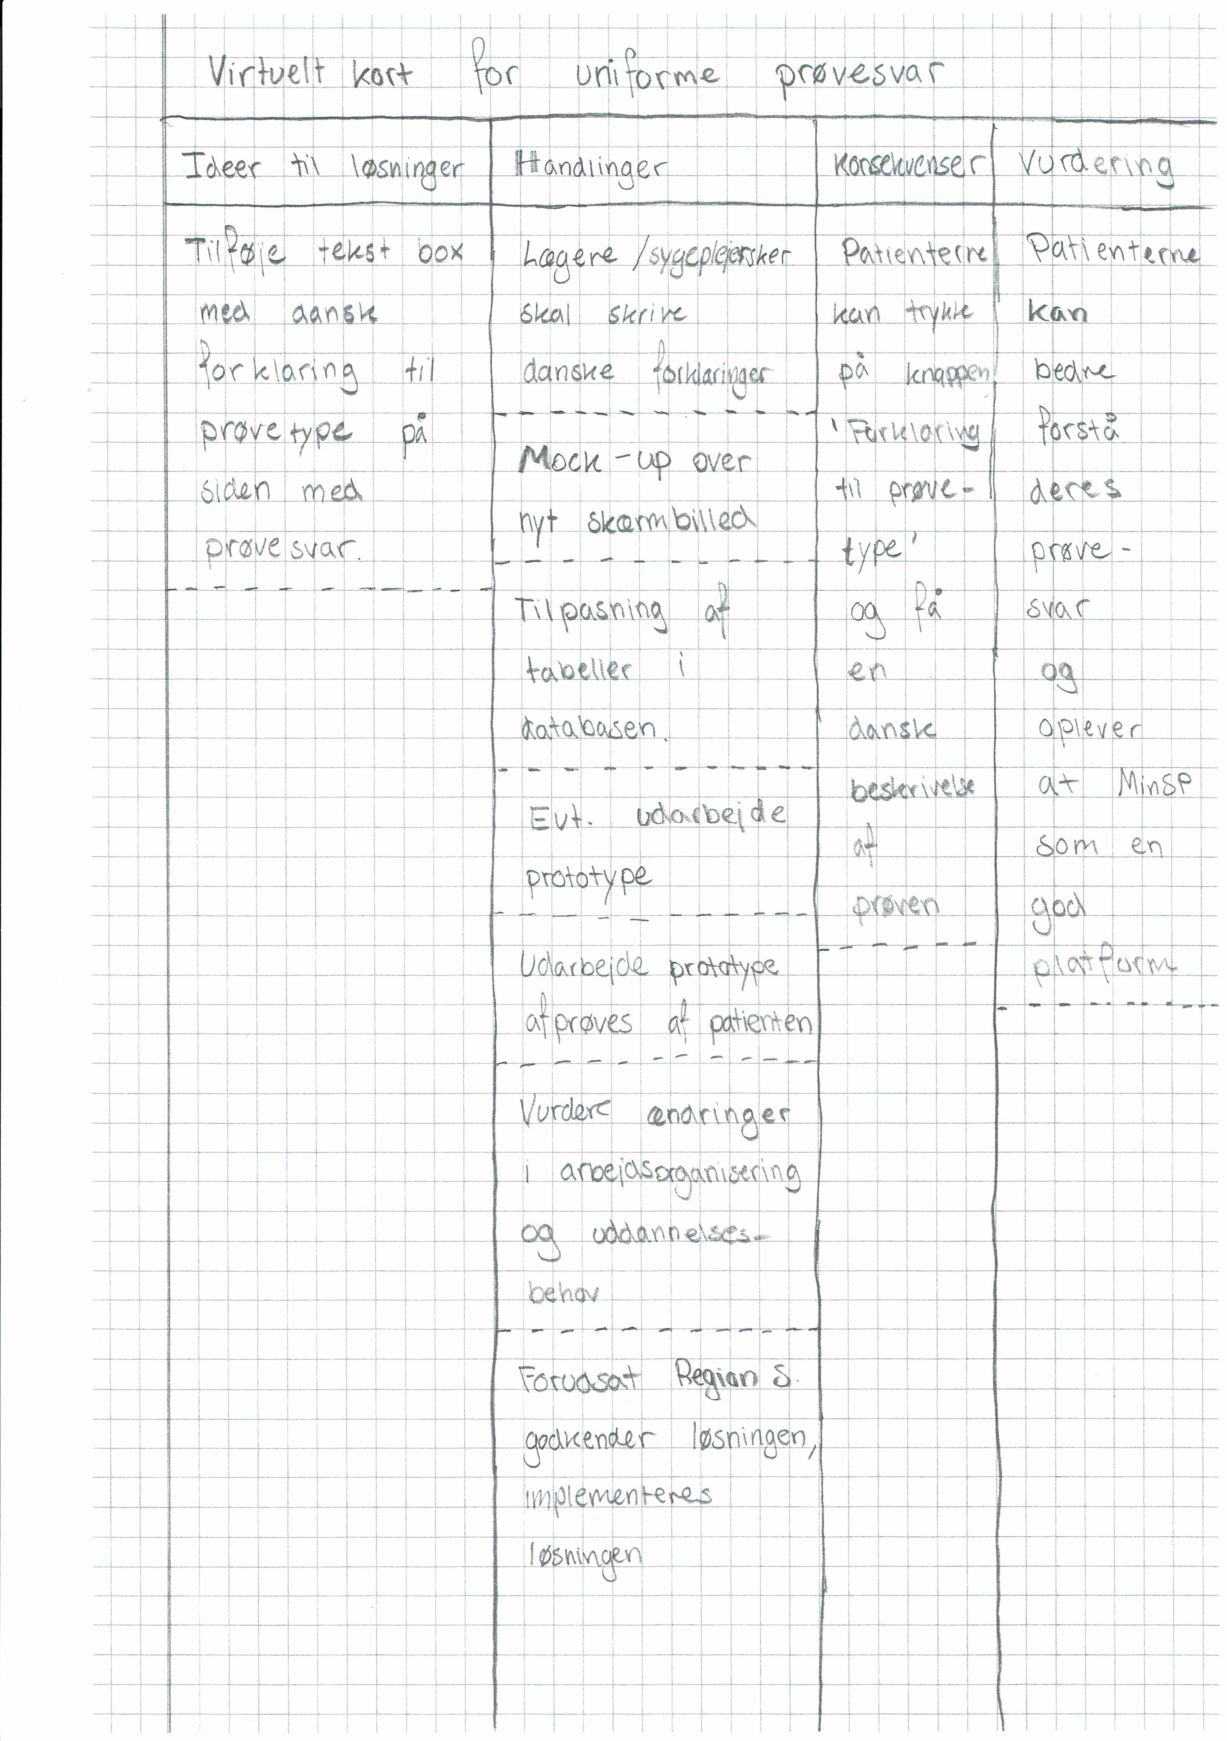
\includegraphics[angle=0, height=0.9\textheight]{Materials/DV_Kort6.pdf}
	%\caption{Mock-up for modulet 'Information om dine diagnoser': Undermenu}
	\label{fig:DVkort6}
\end{figure}
\section{Bilag 4: ER diagram over domænet for MinSP}
\section{ER Diagram}
\begin{figure}[H]
  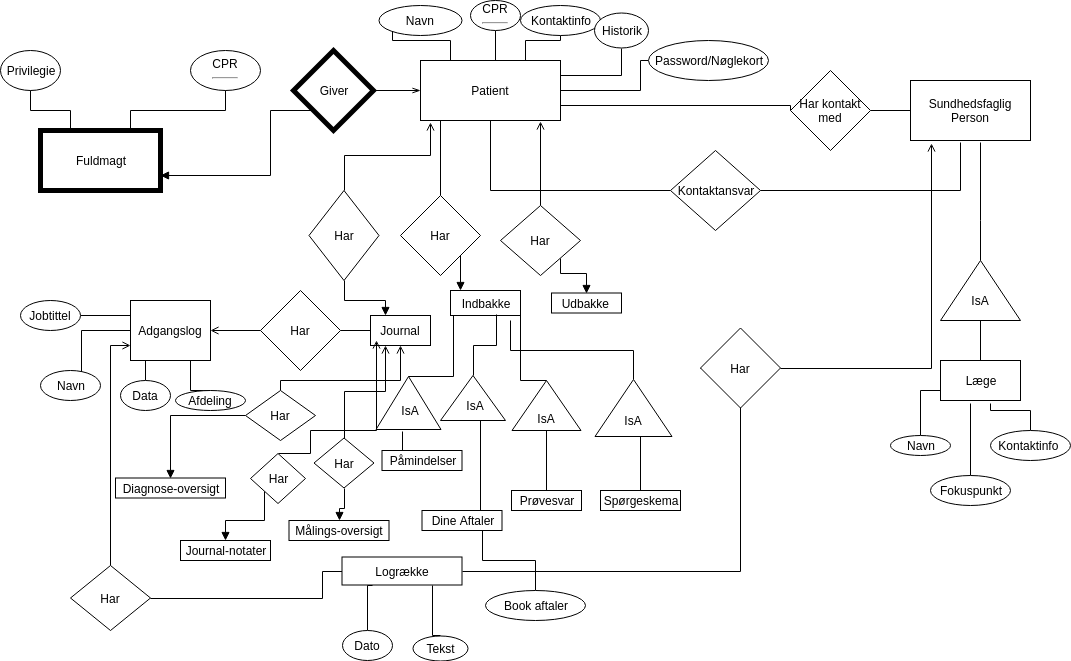
\includegraphics[width=\linewidth]{Materials/ER-diagram.png}
  \caption{ER-diagram for Min Sundhedsplatform}
  \label{fig:ER}
\end{figure}
ER Diagrammet (Ovenstående figur \ref{fig:ER}) viser den logiske model for domænet Min Sundhedsplatform. \\
Entiteterne er de logiske enheder - dvs. aktører, objekter og begivenheder i systemet. 
Relationerne angiver hvilken type af relation, der er mellem entiteterne i systemmet.

Entiteterne angives med rektangler og en tekst typisk et navneord. Til entiteterne er der tilknyttet et eller flere attributter, angivet med en ellipse med en tekst.

Relationerne angives med en diamant med en  tekst, der beskriver relationen mellem to eller flere entiteter.

kardinaliteten beskrives med streger og pile mellem entiteterne. \\ 
En sort lukket pil beskriver: mange til højst en (dvs. 0 eller 1).\\
En åben pil beskriver: mange til præcis en.\\
En streg uden pil beskriver: mange til mange.

Under-entiteter repræsenteres med relationen 'ISA' i en trekant.

En svag entitet er en entitet, der for at relationen kan gælde, kræver at den udover sine egne attributter også skal have sin ejers nøgleattribut som nøgle. Den beskrives med en fed ramme.

Vi kan læse følgende information om Min Sundhedsplatform ud af ER Diagrammet:\\
En patient har tilknyttet attributterne: navn, cpr-nummer, kontakt-info, historik og password/nøglekort. Cpr-nummer er nøgleattribut.\\
Der er en giver-relation fra entiteten patient til entiteten fuldmagt. Der er en mange til en relation, fordi patienten giver fuldmagter og fuldmagterne er givet af én patient. Fuldmagt er en svag entitet, fordi den kræver sin ejers nøgleattribut - dvs. patientens cpr-nummer som nøgleattribut. \\
Patienter har kontakt med mange sundhedsfaglige personer og mange  sundhedsfaglige personer har kontakt ansvar med mange patienter. Læger er under-entitet af sundhedsfaglig personale. \\
Patienten har højest én udbakke, og udbakken tilhører præcis en patient.\\
Patienten har højest én indbakke. Indbakke kan være Påmindelser, Dine Aftaler, Prøvesvar og Spørgeskema.\\
Patienten har højest én journal og en journal tilhører præcis en patient. \\
Journalen har præcis én adgangslog, som har mange logrækker. Logrækken har præcis en adgangslog og præcis en sundhedsfaglig person. En sundhedsfaglig person har mange logrækker.\\
Journalen har én eller ingen diagnose-oversigt og diagnose oversigten tilhører præcis en journal.\\
Journalen har enten ingen eller en journal-notater som tilhører præcis én journal.\\
Journalen har enten én eller ingen målings-oversigt som tilhører præcis én journal.

I designfasen kan den logiske model af ER diagrammet bruges til at danne et overblik over hvilke data, der skal gemmes i systemet, og hvordan flowet er (relationerne mellem entiteterne).\\
ER-diagrammet kan bruges i kommunikationen mellem it-designeren, kunden og brugerne omkring afklaringen af hvilke data, der skal indgå i systemet/domænet. \\
I udviklingsfasen kan ER-diagrammet transformeres til den fysiske model hvor man, ud fra entiteterne, opstiller databaserne/tabeller med de attributter/data, der er behov for i domænet.

%Bilag 4 ER diagram


\end{document}
